\chapter{Image views}
\label{chap:image_views}

\section{The Genesis of a new abstraction layers: Views}

This concept of views is not new and naturally appeared in Image processing with Milena under the name of
morphers~\parencite{levillain.2009.ismm, geraud.2012.hdr}. It was always useful to be able to project an image through a
prism that could extract specific information about it without the need to copy the underlying data buffer. In modern
days, the language C++ (20) also introduce this mechanism with the ranges~\parencite{niebler.2014.ranges} facility for
\emph{non-owning collections}. It is named \emph{views} and allows the user to access a container's content (vector,
map) through a prism. In Pylene, we decided to align the naming system after what was decided in C++20 in order not to
confuse the user. This way, a \texttt{transform} view in image processing will do the same thing on an image that the
transform view in the standard range library does on a container. \emph{Views} feature the following properties:
\emph{cheap to copy}, \emph{non-owner} (does not \emph{own} any data buffer), \emph{lazy evaluation} (accessing the
value of a pixel may require computations) and \emph{composition}. When chained, the compiler builds a \emph{tree of
  expressions} (or \emph{expression template} as used in many scientific computing libraries such as
Eigen~\cite{guennebaud.2010.eigen}), thus it knows at compile-time the type of the composition and ensures a 0-overhead
at evaluation.

There are four fundamental kind of views, inspired by functional programming paradigm: \texttt{transform(input, f)}
applies the transformation $f$ on each pixel of the image \emph{input}, \texttt{filter(input, pred)} keeps the pixels of
\emph{input} that satisfy the predicate \emph{pred}, \texttt{clip(input, domain)} keeps the pixels of \emph{input}
that are in the domain \emph{domain}, \texttt{zip($input_1$, $input_2$, \ldots, $input_n$)} allows to pack several pixel
of several image to iterate on them all at the same time. From those four fundamentals come out more very useful views
such as \texttt{cast<T>(input)} or \texttt{mask(input, msk)} that are more specific to the image processing area.

In Pylena, the fractionner can use a large array of views. Those views comes into different form and allow the
practitioner to seamlessly use arithmetic or logic operators on images like he would using expression template.

\paragraph{The transform view} is the most important view of all. It consists in applying a function to each image's
pixel. For instance, writing the grayscale algorithm with a transform view is as simple as the following code:
\begin{minted}{C++}
  auto grayscale_transform = [](mln::rgb8 val) -> uint8_t {
    return 0.2126 * v[0]    // red
           + 0.7152 * v[0]  // green
           + 0.0722 * v[0]; // blue
  };
  mln::image2d<mln::rgb8> ima_rgb = /* ... */;
  mln::image2d<uint8_t>   ima_grayscale = mln::view::transform(ima_rgb, grayscale_transform);
\end{minted}
There is no loop in this code, just the pixel-wise transformation function. Furthermore, the code will not compute the
resulting image. The computation will happen on-the-fly each time a value from \texttt{ima\_grayscale} is yielded.
This view allows the practitioner to quickly write and adapt any pixel-wise algorithm he needs for his more complex
calculation in an efficient way.

\paragraph{The filter view} is also a fundamental view which consists in keeping only the values that satisfy a
predicate. This is very useful when working with thresholds as shown in the following code:
\begin{minted}{C++}
auto my_threshold = 145;
auto inferior_to [my_threshold](uint8_t val) { return val <= my_threshold; };
auto superiorstrict_to = [](uint8_t val) { return not inferior_to(val); };
mln::image2d<uint8_t> ima_grayscale = /* ... */;
auto ima_inferior = mln::view::filter(ima_grayscale, inferior_to);
auto ima_superiorstrict = mln::view::filter(ima_grayscale, superiorstrict_to);
mln::fill(ima_inferior, 0u8);
mln::fill(ima_superiorstrict, 255u8);
\end{minted}
This code shows a way to binarise \texttt{ima\_grayscale} with a custom threshold using the filter view. It is important
to note that the resulting filtered image has its domain of definition changed. And the new domain of definition will
most likely not be in a regular usual shape (such as a 2D rectangle). This implies that the usage of this view inside
certain algorithms may be limited.

\paragraph{The clip view} is a convenient way to extract a sub-image from a base image. This view essentially redefine
the domain of definition to restrict it into a smaller one. It does not change anything else which means it proxies
every access to the image. For instance, we make use of this view to easily process tiles in an efficient way in the
following code:
\begin{minted}{C++}
  mln::image2d<mln::rgb8> large_image = /* ... */;
  point2d shape = large_image.domain().shape();
  auto chunk_size = 1024;
  auto nb_tile_x = shape.x() / chunks_size + 1;
  auto nb_tile_y = shape.y() / chunks_size + 1;
  for (int x = 0; x < nb_tile_x; ++x)
    for(int y = 0; y < nb_tile_y; ++y) {
      point2D tile_tl { large_image.domain().tl().x() + x*chunk_size,
                        large_image.domain().tl().y() + y*chunk_size };
      point2D tile_bl { large_image.domain().tl().x() + (x+1)*chunk_size,
                        large_image.domain().tl().y() + (y+1)*chunk_size };
      auto tile_domain = mln::box2d{tile_tl,
            tile_bl <= large_image.domain().bl() ? tile_bl : large_image.domain().bl()};
      auto tile = mln::view:clip(ima, tile_domain);
      process_tile(tile);
    }
\end{minted}

\paragraph{The zip view} is one of the most useful view and allow the practitioner to iterate over a set of image at the
same time. The basic use-case consists in iterating over a set of input image and the output image to be able to
consistently assign output values to a resulting computation from input values. Its usage is shown in the following
code:
\begin{minted}{C++}
  mln::image2d<uint8_t> input = /* ... */;
  mln::image2d<uint8_t> output{input.domain()};
  auto zipped_ima = mln::view::zip(input, output);
  for (auto&& [v_in, v_out] : zipped_ima.values())
    v_out = v_in < 145 ? 0 : 255; // binarisation
\end{minted}
This code is another example of how to compute a binary threshold image.

\paragraph{The mask view} is very image-processing oriented as it allows the practitioner to provide a boolean image the
same size as the original image to select only the pixels whose corresponding value in the mask is true. Its usage is
shown in the following code:
\begin{minted}{C++}
  mln::image2d<mln::rgb8> ima = /* ... */;
  auto mask = ima > 127;
  mln::fill(mln::view::mask(ima, mask), 255);
\end{minted}
This code set all the values that are superior to 127 to the max value 255. It shows that it can both be used with read
and write access.

\paragraph{The channel/RGB views} is a projector to access a specific color channel of an image. There exists image with
many more channels than just the standard red/green/blue ones, from the astrophysics or medical area for instances. This
view is a tool to restrict an image and only access a specific channel. Its usage is shown in the following code:
\begin{minted}{C++}
  mln::image2d<mln::rgb8> ima = /* ... */;
  mln::copy(mln::view::red(ima), mln::view::green(ima));
\end{minted}
This code copies the red component into the green component. It shows that the view can be used in both read and write
access. Another more generic view exists; \mintinline{c++}{mln::view::channel(ima, k)}, that access the \texttt{k}-th
channel in \texttt{ima}.

\paragraph{The cast views} is a way to convert an image's underlying type to another type, by performing a cast. As this
does not modify the underlying value in itself, the access cannot be a write access. This view can be used as shown in
the following code:
\begin{minted}{C++}
  mln::image2d<double> ima = /* ... */;
  mln::image2d<uint8_t> ima_8bits = mln::view::cast<uint8_t>(ima);
\end{minted}

\paragraph{The arithmetical operators} $+, -, *, /, \%$ are implemented in the form of transformation views that operate
point-wise between two images whose size is identical. For instance, writing the following code:
\begin{minted}{C++}
  mln::image2d<uint8_t> ima1 = /* ... */;
  mln::image2d<uint8_t> ima2 = /* ... */;
  auto ret = ima1 + ima2;
\end{minted}
Is equivalent to writing the following code:
\begin{minted}{C++}
  auto ret = mln::view:transform(ima1, ima2, [](auto v1, auto v2){ return v1 + v2; });
\end{minted}
It is important to note that the \texttt{-} unary operator is also supported: \mintinline{C++}{-ima1}.

\paragraph{The logical operators} $<, <=, ==, !=, >, >=$ are implemented in the same way that arithmetical operators
are. Both unary and binary operators are expressed as transform views such as writing the following code:
\begin{minted}{C++}
  auto ret = !ima1 && ima2;
\end{minted}
is equivalent to writing the following code:
\begin{minted}{C++}
  auto tmp = mln::view::transform(ima1, [](auto v){ return !v; });
  auto ret = mln::view::transform(tmp, ima2, [](auto v1, auto v2){ return v1 && v2; });
\end{minted}
It is far more expressive and more comprehensible by the practitioner. Also, a new facility is introduced to express the
logic behind a ternary expression (if C then A else B): the operator $ifelse(C, A, B)$. The rationale is to be able to
swap between values depending on a boolean mask. This way, a mathematical morphology algorithm such as \emph{hit or
  miss} can be implemented in the following simple manner:
\begin{minted}{C++}
  mln::image2d<uint8_t> ima = /* ... */;
  auto ero = erode(ima);
  auto dil = dilate(ima);
  uint8_t zero = 0;
  auto ret = mln::view::ifelse(dil < ero, ero - dil, zero);
\end{minted}
Everything is taken care of and the practitioner just has to write down his algorithm to get it done.

\paragraph{The mathematical operators} are implemented in the form of views that operates point-wise. The supported
mathematical operators are the following: abs, pow, sqr, cbrt, sqrt, sum, prod, min, max, dot, cross, l0norm, l1norm,
l2norm, l2norm\_sqr, linfnorm, lpnorm, l0dist, l1dist, l2dist, l2dist\_sqr, linfdist, lpdist. Calling an operator onto
an image is equivalent to calling a transform view on each value of this image:
\begin{minted}{C++}
  auto ima = /* ... */;
  auto ret = view::maths::abs(ima);
\end{minted}
Is equivalent to calling:
\begin{minted}{C++}
  auto ima = /* ... */;
  auto ret = view::transform(ima, [](auto v){ return std::abs(v); });
\end{minted}


\section{Upgrading the way to design IP algorithms}

As seen in~\cref{chap:image.algorithms.taxonomy}, there are three main categories of algorithms. First there are the
\emph{pixel-wise} algorithms which perform operations for each pixel without knowing about the other pixels. Second,
there are the \emph{local} algorithms which perform an operation on a pixel with the knowledge of a window of pixels
around this pixel. Finally, there are \emph{global} algorithms which perform an operation on a pixel with the knowledge
of the whole image. \emph{Views} introduce an abstraction layer that is able to completely handle the first case:
pixel-wise algorithm. Indeed, every pixel-wise loop can be rewritten using the four fundamental views. This is not the
case for local and global algorithms though.

Another key point to note is the lazy-evaluation. Indeed, often an IP practitioner will transform a whole image and
only make use of a small subpart of it. Thanks to the lazy-evaluation property, only the exploited subimage will be
transformed on-the-fly at the call site. However, if there are several call site browsing the view the same way, it can
incur a performance loss as the same calculation is performed several time, each time the image is browsed. In this
case, it is better to create a temporary concrete subimage (with a data buffer) that contains the values that will be
asked several times.

The other key part about \emph{views} is the composability. Image processing is an area in which a practitioner design
pipelines which, by nature compose several operations on top of each other. Views have the ability to be composable with
each others to get the wanted result.

Finally, a view is a \emph{non-owning} and \emph{cheap-to-copy} image, and that design has consequences on its usage.

\subsection{Data ownership}

The concept of \emph{View} brought to us a fundamental issue when dealing with images: \blockquote{\emph{What is an
    image?}}. More precisely: should an image always be the owner of its data buffer? Should we have a shared ownership of
the data buffer between all the images using it? Then what happens when the data changes? The issue about the semantic
of an image is crucial but also very similar to the issue there is to differentiate a \emph{container} (such as
\texttt{std::vector}, that is to say the data buffer) and a \emph{view} on this container in the \emph{Ranges TS}.

From here we have considered two approaches. The first one is to have \emph{shared ownership} of the data buffer for the
image and its derived views. However this does not allow the differentiation between an already computed image and a
lazy image. To be able to make this differentiation is crucial in an \emph{Image Processing library} as we want to make
the most out of the data we already have and we do not want to compute data we do not need. Also, we cannot distinguish
when the \emph{copyability} property is required. This is the main reason why we did not adopt this approach.

The second one is to make the differentiation between a \emph{concrete image} which owns the data (like the standard
containers) and the \emph{views} that are lightweight cheap-to-copy objects. Not all \emph{concrete image} may be
\emph{copyable}, but all \emph{views} are. This is a very important property as it simplify greatly the reasoning when
performance is needed. It also enables us to have a library design similar to the standard library which the user is
familiar with and, why not, have standard algorithm and standard view work on our images types. All of these are the
main reason why we decided to adopt this design. Henceforth from now on the \emph{Image} concept is similar to the
\emph{View} concept from which we refines a \emph{ConcreteImage} concept that requires a specific behavior as it owns
data.


In (subsec.gen.concept), we saw that what is truly important is the behavior: an algorithm will require its input to be
able to behave a certain way, and if those requirements are fulfilled, then the algorithm can be used with this set of
inputs. This enables non-standard type of image to be input in algorithms, providing they still behave correctly. The
way how we can check if the required behavior is satisfied is a new C++20 feature called \emph{concept} (the authors
show how to leverage them in~\cite{roynard.2019.rrpr}) that will not be presented in this paper. Additionally to
concepts, C++20 introduces a new library facility called
\emph{ranges}~\cite{niebler.2018.deepranges,niebler.2018.mergingranges} which includes a non-owning lightweight
container called \emph{views} whose design is very similar to that of \emph{morphers}, introduced in
Milena~\cite{levillain.2009.ismm,geraud.2012.hdr}. Views are completely transferable to the image processing world.
Also, views feature interesting properties that an image processing practitioner will find to his taste.

A view is a \emph{lightweight object} that behaves exactly the same as an image: let $V$ be a view of an image defined
on $\mathcal{D}$ then we have $\forall{p}\in\mathcal{D}, v = V(p)$. It can be a random generator that yields a random
number each time $V(p)$ is called; a proxy to the underlying image that records the number of times each pixel is
accessed in order, for instance, to compare algorithm performance; a projection to a specific color channel; applying an
automatic gamma correction; restricting the definition domain $\mathcal{D}$; and so on.

A view is a \emph{non-owning}, \emph{cheap-to-copy} lightweight object that basically only \emph{records an
  operation} and stores a pointer to an image. For instance, let us consider the view transform defined as follow $v =
  transform(u_1, u_2, \cdots, u_n, f)$ where $u_i$ are input images and $h$ a n-ary function. $transform$ returns an image
generated from the other image(s) as show in~\cref{fig.view.threshold}. Also, we can see that the view itself does not
own any image but just stores pointers as well as the operation ($h$). This means that, for instance, modifying the
original values of the image(s) will impact the values yield by the view. Finally, as the view is cheap-to-copy, it
features a pointer semantic that help the practitioner passing around his images by copy to his algorithms without
worrying about heavy buffer copies in the background.

\begin{figure}[tbh]
  \centering
  \begin{minipage}{\linewidth}
    \includestandalone[mode=image, width=.9\linewidth]{figs/transform_thresholding}
  \end{minipage}
  \caption{An image view performing a thresholding.}
  \label{fig.view.threshold}
\end{figure}

\subsection{Lazy evaluation, composability and piping}
\label{subsec:image.views.lazy.eval}

Another key point of views is the lazy evaluation. When an image is piped through a view, no computation is done. The
computation happens when the practitioner requests a value by doing $val = V(p)$. The implications are multiples: an
image can be piped into several computation-heavy views, some of which can be discarded later on, it won't impact the
performance. Also, when processing large images, applying a transformation on a part of the image is as simple as
restricting the domain with a view and applying the transformation to this resulting sub-image.

\emph{Lazy-evaluation} combined with the view \emph{chaining} allows the user to write clear and very efficient code
whose evaluation is delayed till very last moment as shown in~\cref{fig.lazy} (see \cite{geraud.2018.gtgdmm} for
additional examples). Neither memory allocation nor computation are performed; the image $i$ has just recorded all the
operations required to compute its values.

\begin{figure}[htbp]
  \begin{minipage}[l]{0.48\linewidth}
    \begin{minted}{C++}
image2d<rgb8>  ima1 = /* ... */;
image2d<uint8_t> ima2 = /* ... */;

// Projection: project the red channel value
auto f = view::transform(ima, [](auto v) {
  return v.r;
});

// Lazy-evaluation of the element-wise
// minimum
auto g = view::transform(view::zip(f, ima2),
  [](auto value) {
    return std::min(std::get<0>(value),
             std::get<1>(value));
});
\end{minted}
  \end{minipage}
  \hfill
  \begin{minipage}[l]{0.48\linewidth}
    \begin{minted}{C++}
// Lazy-Filtering: keep pixels whose value
// is below < 128
auto h = view::filter(g, [] (auto value) {
  return value < 128;
}));

// Lazy-evaluation of a gamma correction
using value_t = typename Image::value_type;
constexpr float gamma = 2.2f;
constexpr auto max_val =
  std::numeric_limits<value_t>::max();
auto i = view::transform(h,
  [gamma_corr = 1 / gamma] (auto value) {
    return std::pow(value / max_val,
             gamma_corr) * max_val;
});
\end{minted}
  \end{minipage}

  \caption{Lazy-evaluation and \emph{view} chaining.}
  \label{fig.lazy}
\end{figure}

\noindent The tree of type resulting from this view chaining is illustrated by~\cref{fig.viewAST}.

\begin{figure}[htb]
  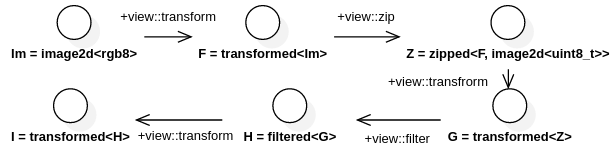
\includegraphics[height=2cm]{figs/viewAST.png}
  \caption{Abstract Syntax Tree of the types chained by the code above}
  \label{fig.viewAST}
\end{figure}

Views will also try to preserve properties of the original image when they can. That means that views can preserve the
ability of the practitioner to, for instance, write into this image. This may be a trivial property to preserve when
considering a view that restrict a domain, but when considering a view that transforms the resulting values, it is not.
Let us consider the projection $h: (r,g,b) \mapsto g$ that selects the green component of an RGB triplet. When piping
the resulting view into, for instance, a blurring algorithm, the computation will take place in place thanks to still
having the ability to write into the image. A legacy way of obtaining the same result would have been to create a
temporary single-channel image consisting of the green channel of the original RGB image so that the temporary image
could then be blurred. Then one would have needed to copy the values of the temporary image back into the green channel
of the original image. The comparison between the legacy way and the in-place way of doing this computation is shown
in~\cref{fig.legacy.vs.view}.

\begin{figure}[tbh]
  \centering
  \subfloat[Legacy pipeline with copy]{
    \includegraphics[width=1.6in,align=t]{figs/blur_copy}
  }
  \hfil
  \subfloat[Modern pipeline with view]{
    \includegraphics[width=1.6in,align=t]{figs/blur_inplace}
  }

  \caption{Comparison of a legacy and a modern pipeline using \colorbox{lightgreen}{algorithms} and
    \colorbox{thistle}{views}.}
  \label{fig.legacy.vs.view}
\end{figure}

On the other hand, when considering the view $g: (r,g,b) \mapsto 0.2126*r+0.7152*g+0.0722*b$ that compute the gray level
of a color triplet (as shown in~\cref{fig.view.grayscale}), the ability to write a value into the image is not
preserved. One would need an inverse function that is able to deduce the original color triplet from the gray level to
be able to write back into the original image.

\begin{figure}[tbh]
  \centering
  \includegraphics[width=.98\linewidth]{figs/views/transform_grayscale}
  \caption{Usage of transform view: grayscale.}
  \label{fig.view.grayscale}
\end{figure}

\begin{figure}[tbh]
  \includestandalone[mode=image, scale=0.6]{figs/clip}

  \includestandalone[mode=image, scale=0.6]{figs/filter}
  \caption{Clip and filter image adaptors that restrict the image domain by a non-regular ROI and by a predicate that
    selects only even pixels.}
  \label{fig.view.clip}
\end{figure}

Following the same principle, a view can apply a restriction on an image domain. In~\cref{fig.view.clip}, we show the
adaptor \texttt{clip(input, roi)} that restricts the image to a non-regular \texttt{roi} and \texttt{filter(input,
  predicate)} that restricts the domain based on a predicate. All subsequent operations on those images will only affect
the selected pixels.

\begin{figure}[tbh]
  \includestandalone[mode=image, scale=0.6]{figs/pipeline}
  \caption{Example of a simple image processing pipeline.}
  \label{fig.view.pipeline}
\end{figure}

Views feature many interesting properties that change the way we program an image processing application. To illustrate
those features, let us consider the following image processing pipeline: (Start) Load an input RGB-8 2D image (a
classical HDR photography) (A) Convert it in grayscale (B) Sub-quantize to 8-bits (C) Perform the grayscale dilation of
the image (End) Save the resulting 2D 8-bit grayscale image; as described in~\cref{fig.view.pipeline}.


\begin{figure}[tbh]
  \begin{minipage}{\linewidth}
    \includestandalone[mode=image, scale=0.59]{figs/composition}
  \end{minipage}
  \caption{Algorithm vs image view composition.}
  \label{fig.view.comp}
\end{figure}

\subsection{Keeping properties}

While is it tempting to use views everywhere, it is also important to note that you may converse or loose some
properties from the base concrete image (the one holding the data buffer). To give a quick example, let us consider a
classic RGB image and a view that calculate the grayscale on-the-fly. When only seeing the view, it is not possible to
modify the base values which are RGB colors. Indeed, we cannot infer how a modification on the grayscale value will
impact the base color of the image. Passing from a grayscale image to a colored image is a research area on its own and
cannot be done deterministically on-the-fly in a fixed time. This induces that piping an image into this grayscale views
turns the image \emph{read-only}. in this case, The image loose the ability to be mutable. Another case would be a view
that performs a projections of one of the color channel. This way the resulting viewed image is still mutable and
modifying its values would only modify the color channel projected. Keeping properties is not an easy subject and
requires the attention of the practitioner to pipe the correct operations to keep the properties he wants to keep.

There are six properties one want to keep track when working with views: forward, bidirectional, raw, writable,
accessible and indexable. Those properties echo to the concepts seen in~\cref{sec:library.concepts}. And image is
\emph{forward} when it can be traversed in a forward way. It is \emph{bidirectional} when it can be traversed in both a
forward and a backward way. It is \emph{raw} when its data buffer can is contiguous and can directly be accessed with
information about strides. It is \emph{writable} when the values are mutable. It is accessible whenever it allows to
access the value associated to a point (i.e. it allows to write the expression $v = ima(p)$). Finally, an image is
\emph{indexable} whenever its values can be accessed through an index localisator (i.e. it allows to write the
expression $v = ima[idx]$). Usually, accessing through an index is faster than accessing by a point. The
table~\cref{table:views.properties} present all the views and how they conserve the base properties of a concrete image.

\begin{table}[tbh]
  \begin{scriptsize}
    \begin{threeparttable}
      \caption{Views: property conservation}
      \begin{tabular}{|l|l|cccccc|}
        \hline
        \thead{View type}    & \diagbox{\thead{Expression}}{\thead{Property}} & Forward & Bidirectional & Raw    & Writable   & Accessible & Indexable \\
        %\thead{View type}    & \thead{Expression | Properties:} & Forward & Bidirectional & Raw    & Writable   & Accessible & Indexable \\
        \hline
        \thead{Image}        & \texttt{ima1, ima2}                            & \cmark  & \cmark        & \cmark & \cmark     & \cmark     & \cmark    \\
        \thead{Cast}         & \texttt{cast<T>(ima)}                          & \cmark  & \cmark        & \xmark & \xmark     & \cmark     & \cmark    \\
        \thead{Transform}    & \texttt{transform(ima, func)}                  & \cmark  & \cmark        & \xmark & \cmark$^1$ & \cmark     & \cmark    \\
        \thead{Filter}       & \texttt{filter(ima, pred)}                     & \cmark  & \cmark        & \xmark & \xmark     & \cmark     & \cmark    \\
        \thead{Clip}         & \texttt{clip(ima, dom)}                        & \cmark  & \cmark        & \xmark & \cmark     & \cmark     & \cmark    \\
        \thead{mask}         & \texttt{mask(ima, mask)}                       & \cmark  & \cmark        & \xmark & \cmark     & \cmark     & \cmark    \\
        \thead{Zip}          & \texttt{zip(ima1, ima2)}                       & \cmark  & \cmark        & \xmark & \cmark     & \cmark     & \cmark    \\
        \thead{Channel}      & \texttt{red(ima)}                              & \cmark  & \cmark        & \xmark & \cmark     & \cmark     & \cmark    \\
        \thead{Arithmetic}   & \texttt{ima1 + ima2}                           & \cmark  & \cmark        & \xmark & \xmark     & \cmark     & \cmark    \\
        \thead{Logical}      & \texttt{ima > 125}                             & \cmark  & \cmark        & \xmark & \xmark$^2$ & \cmark     & \cmark    \\
        \thead{Mathematical} & \texttt{abs(ima)}                              & \cmark  & \cmark        & \xmark & \xmark     & \cmark     & \cmark    \\
        \hline
      \end{tabular}
      \begin{tablenotes}
        \item $^1$: writability is preserved only if \texttt{func} is a projection.
        \item $^2$: writability not preserved except for the expression \texttt{ifelse(ima, ima1, ima2)}.
      \end{tablenotes}
      \label{table:views.properties}
    \end{threeparttable}
  \end{scriptsize}
\end{table}

\subsection{Summary}

\textbf{Views are composable.} Chaining operations has always been a very important feature in image processing as well
as in software engineering in general (known object composition). Being able to weave simple blocks together into more
complex blocks in a way that the resulting block can still be treated as a simple block is a most wanted feature.
The~\cref{fig.view.pipeline} features an example of a pipeline using 3 basic operations \emph{Image} $\rightarrow$
\emph{Image}: a grayscale conversion, a sub-quantization and a dilation. It is important to note that we can consider
there is only one complex operation composed of 3 basic algorithms in which an image is piped. A view thus carries both
information about the image and the transformations. In~\cref{fig.view.comp} we show the distinction between the
composition of algorithms and the compositions of views which carry both the image and the transformations.

\textbf{Views improve usability.} The code featuring the pipeline in~\cref{fig.view.comp} can almost be implemented the
following way:
\begin{minted}{c++}
auto input = imread(...);
auto A = transform(input, [](rgb16 x) -> float {
    return (x.r + x.g + x.b) / 3.f; };
auto MyComplexImage = transform(A, [](float x)
    -> uint8_t { return (x / 256 + .5f); };
\end{minted}
When one is familiar to functional programming, it is quite easy to draw the parallel between \emph{transform},
\emph{map}, \emph{filter} and the sequence operators. Views are, in reality, higher-order functions built from an image
as well as the function(s) (operator or predicate) to apply for each pixel. It is not required to make the iteration
over each pixel of the image oneself, we just provide the function to morph the image into another one. The technique
used when composition several sequence operators is called \emph{currying}~\cite{hanus.1995.curry} in the functional
programming world.

\textbf{Views improve re-usability.} When looking at the code snippets above, one could see that they are simple though
not very re-usable. However, keeping the functional programming paradigm in mind, one can easily define new views just
by considering that a view is a \emph{higher-order function}. Then, as shown in~\cref{fig.view.highorder}, the primitive
\emph{transform} serves as the basis to build three new views: one that performs the summation of two images, one that
performs the grayscale conversion and one that performs the sub-quantization. All those three views can then be reused
afterwards\footnote{A more generic implementation could have been provided for these views for even more re-usability,
  but this is not the purpose here.}.

\begin{figure}
  \noindent
  \begin{minted}{c++}
auto operator+(Image A, Image B) {
  return transform(A, B, std::plus<>());
}
auto togray = [](Image A) { return transform(A, [](auto x)
  { return (x.r + x.g + x.b) / 3.f; };)
};
auto subquantize16to8b = [](Image A) { return transform(A,
  [](float x) { return uint8_t(x / 256 +.5f); });
};

auto input = imread(...);
auto MyComplexImage = subquantize16to8b(togray(A));
  \end{minted}

  \caption{Using high-order primitive views to create custom view operators.}
  \label{fig.view.highorder}
\end{figure}

\textbf{Views for lazy computing.} One fundamental point of views is that they embed the operation within themselves,
meaning that in~\cref{fig.view.highorder}, the creation of the views does not incur any computation. The computation is
delayed until the invocation of the \texttt{v(p)} expression. Also, the computation can be delayed quite far thanks to
the composition capability of views. In fact, a view is an image adaptor which actually is a \emph{template
  expression}~\parencite{veldhuizen.1995.expression, veldhuizen.2000.blitz}. Indeed, the \emph{expression} used to
generate the image is recorded as a template parameter. A view is represented by an \emph{expression tree}, as shown
in~\cref{fig.view.ast}.


\begin{figure}
  \null\hfill
  \begin{minipage}[b]{2cm}
    \includestandalone[mode=image, scale=0.8]{figs/view_ast}
  \end{minipage}
  \begin{minipage}[b]{5.5cm}
    \begin{minted}{c++}
Image f = ...; // grayscale
Image g = ...; // rgb16
Image out = subquantize16to8b(
              togray(g)) + f;
\end{minted}
  \end{minipage}
  \caption{View composition seen as an expression tree.}
  \label{fig.view.ast}
\end{figure}


\section{A practical example: border management}

\label{sec:border.management}

When looking at local algorithms, we notice that a long recurring issue is about the behavior on the border of the
image. There are many ways of dealing with this problem. One is to allocate additional memory for the border and paste
values in it. Another is to check the bounds when looping over the neighbors inside the computational window. We can
also decorate the image to return a correct lazily computed value when accessing out-of-image's-bound value still inside
the extension. The point is: all these methods have advantages as well as disadvantages.

\paragraph{Memory allocated border}
The border width is fixed at the image's creation and cannot be augmented without doing a reallocation. There is also a
cost when computing border's values (to fill it) which is proportional to the border's width and to the image's size. On
the other hand, the access time of a border value during the algorithm unrolling is as fast as a native access time
within the image itself. The last issue remaining would be that the border is not infinite. We cannot process a local
algorithm with a structuring element that does not fit in the extension. This method is especially adapted when there is
medium structuring elements with a known size which will yield a lot of out-of-image's bound accesses. When speed is
required, this method is a de facto standard.

\paragraph{Bound checking}
Assuming there is no border and we are not allowed to access out-of-image's-bound values, a bound check is required when
accessing each values. Another way to do would be to decorate the facility that yields the neighbors of a pixel: do not
yield out-of-image's-bound pixels. This removes the need to bound check for each pixel's value which is relatively
faster. The caveats of this method are that it induces a slight slow down when yielding the pixel's neighbors from the
structuring element, and that it is not always viable: some algorithms do need to access values in an extension to
produce proper results.

\paragraph{Image decoration}
The border is infinite and we make a view of our image to decorate it with the required extension. This method has the
advantage to \textit{always work}. Given any structuring element of any size, any algorithm will work. The disadvantage
is that we need to check for out-of-bound access at the image level, and lazily compute the value in case of
out-of-image's-bound access. The slowness induced is not negligible and should be weighted carefully.

\bigskip

It is important to note the very close relation between an image's domain (to perform out-of-bound checks), the
structuring element (notably its size) and the extension (its width). A user may require, for a specific set of those
three elements, to decorate the image, and/or the structuring element and/or to perform computation and/or reallocation.
To resolve this issue, we decided to provide the user with a new facility: the \textit{border manager} whose job is to
prepare a suitable pair (image and structuring element) given a set of configuration wanted by the user.

We designed the configuration to be constructed from a given set of a policy and a method. We currently offer two
policies: native and auto.

\begin{itemize}
  \item Native: if the border is large enough: forward the image as-is to the algorithm to allow the fastest access
        possible. Otherwise, the border manager fails and halt the program.
  \item Auto: if the border is large enough: forward the image as-is to the algorithm to allow the fastest access
        possible. Otherwise, decorate the image with a view whose extension will emulate what is required by the
        algorithm with the given structuring element.
\end{itemize}

We also provide seven different methods to fill up our extension with the wanted values. It is important to note that
not all the methods are available for both policies. The policies are: none, fill, mirror, periodize, clamp, image and
user.

\paragraph{None} Enforces enforce a policy where there is no border to use. The method cannot fail as it enforces the
border to vanish. To enforce this method, the border manager decorate the structuring element in a view that checks the
domain inclusion of each neighboring point. And example is given in figure~\ref{fig:border.none}.

\begin{figure}[tbh]
  \centering
  \includegraphics[width=1in]{figs/extensions/none}
  \caption{Border method: none.}
  \label{fig:border.none}
\end{figure}

\paragraph{Fill} Enforces that the border is filled with a specific value. The figure~\ref{fig:border.fill} shows an
image whose border is filled with the value $0$.

\begin{figure}[tbh]
  \centering
  \includegraphics[width=2in]{figs/extensions/fill}
  \caption{Border method: fill.}
  \label{fig:border.fill}
\end{figure}

\paragraph{Fill} Enforces that the border is filled with a mirrored value from an axial symmetry relative to the image's
edges. The figure~\ref{fig:border.mirror} shows an image whose border is filled with mirrored values.

\begin{figure}[tbh]
  \centering
  \includegraphics[width=2in]{figs/extensions/mirror}
  \caption{Border method: mirror.}
  \label{fig:border.mirror}
\end{figure}

\paragraph{Periodize} Enforces that the border replicate the image, like a mosaic. The
figure~\ref{fig:border.periodize} shows an image whose border is filled with periodized values.

\begin{figure}[tbh]
  \centering
  \includegraphics[width=2in]{figs/extensions/periodize}
  \caption{Border method: periodize.}
  \label{fig:border.periodize}
\end{figure}

\paragraph{Clamp} Enforces that the border is filled with values expanded from the values at the image's edge. The
figure~\ref{fig:border.clamp} shows an image whose border is filled with clamped values.

\begin{figure}[tbh]
  \centering
  \includegraphics[width=2in]{figs/extensions/clamp}
  \caption{Border method: clamp.}
  \label{fig:border.clamp}
\end{figure}

\paragraph{Image} Enforces all points out of the current image's domain are to be picked inside another image. A basic
use-case is preparing tiles from a large image. The position of our image can be offset in the image acting as an
extension which ease the ease of usage. The figure~\ref{fig:border.image} shows how a subimage (tile) can consider the
base image as its border.

\begin{figure}[tbh]
  \centering
  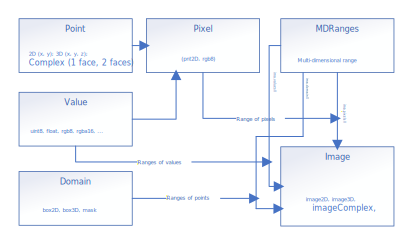
\includegraphics[width=2in]{figs/extensions/image}
  \caption{Border method: image.}
  \label{fig:border.image}
\end{figure}


\paragraph{User} Assumes the user knows what he is doing and do not touch nor decorate the given image in any way. Both
policies lead to the same behavior: check whether the structuring element fit and then forward the image as-is if it
fits. An exception is raised if it does not.

As a consequence the usage of a local algorithm becomes very simple:

\begin{minted}{C++}
  // default border width is 3
  image2d<int> ima = {{0, 1, 0}, {0, 1, 1}, {0, 1, 0}};
  auto disc_se = se::disc{1}; // radius is 1
  auto bm = extension::bm::fill(0); // fill border with 0 with policy auto

  local_algorithm(ima, disc_se, bm); // will handle the border for you
\end{minted}

The border manager \texttt{bm} is set with the method fill (with value 0) and policy \texttt{auto} (wich is the default
policy). To use the policy \texttt{native}, one would write \texttt{extension::bm::native::fill(0)} instead.

In the implementation of the local algorithm, a dispatch is made with the pattern \emph{visitor}, relying on the
standard facilities \texttt{std::visit} and \texttt{std::variant} so that the performance overhead as well as the
complexity of use remain minimal. Let us assume we have a local algorithm implemented this way:
\begin{minted}{C++}
  template <class Ima, class SE>
  local_algorithm(Ima ima, SE se)
  {
    // assume ima has a large enough border for the given se
    // use ima & se in loop
  }
\end{minted}
We can rewrite it leveraging the border manager facility this way :
\begin{minted}{C++}
  template <class Ima, class SE, class BM>
  local_algorithm(Ima ima, SE se, BM bm)
  {
    auto [managed_ima, managed_se] = bm.manage(ima, se);
    std::visit([&](auto&& ima_, auto&& se_) { 
      // use ima_ & se_ in loop
     }, managed_ima, managed_se);
  }
\end{minted}
The overhead is kept minimal thanks to using \texttt{std::variant} and \texttt{std::visit} and the algorithm implementer
delegate the border management to the border manager. This is made possible thanks to the views. Indeed, under the hood
the border manager may pipe the orginal image into a view that will behave accordingly to the policy chosen by the user.
This will be transparent from both practitioner and maintener points of views.


\section{Performance discussion}

In order to have a relevant discussion on performances, we decided to implement a real world image processing pipeline:
the background subtraction. It is used to detect changes in image sequences~\cite{opencv.bg_sub}. It is mainly used when
regions of interest are foreground objects. The pipeline components include: subtraction, Gaussian filtering, threshold,
erode and dilate, as shown in~\ref{fig.view.comp.sub_bg}.

\begin{figure}[tbh]
  \begin{minipage}{\linewidth}
    \includestandalone[mode=image, scale=0.59]{figs/pipeline_bg_sub_comp}
  \end{minipage}
  \caption{Background substraction pipeline using \colorbox{lightgreen}{algorithms} and
    \colorbox{thistle}{views}.}
  \label{fig.view.comp.sub_bg}
\end{figure}

We have decided to run the algorithm on an original set of image to detect a changing foreground. Here are the 10 sets
we have considered.

\paragraph{Set \#1: castle} The figure~\ref{fig:bg_sub.castle.restults} presents the first candidate set we have run
the algorithm with.

\begin{figure}[tbh]
  \centering
  \begin{tabular}{cccc}
    Background
                                                                                     & Candidate & Result \\[5pt]
    \fbox{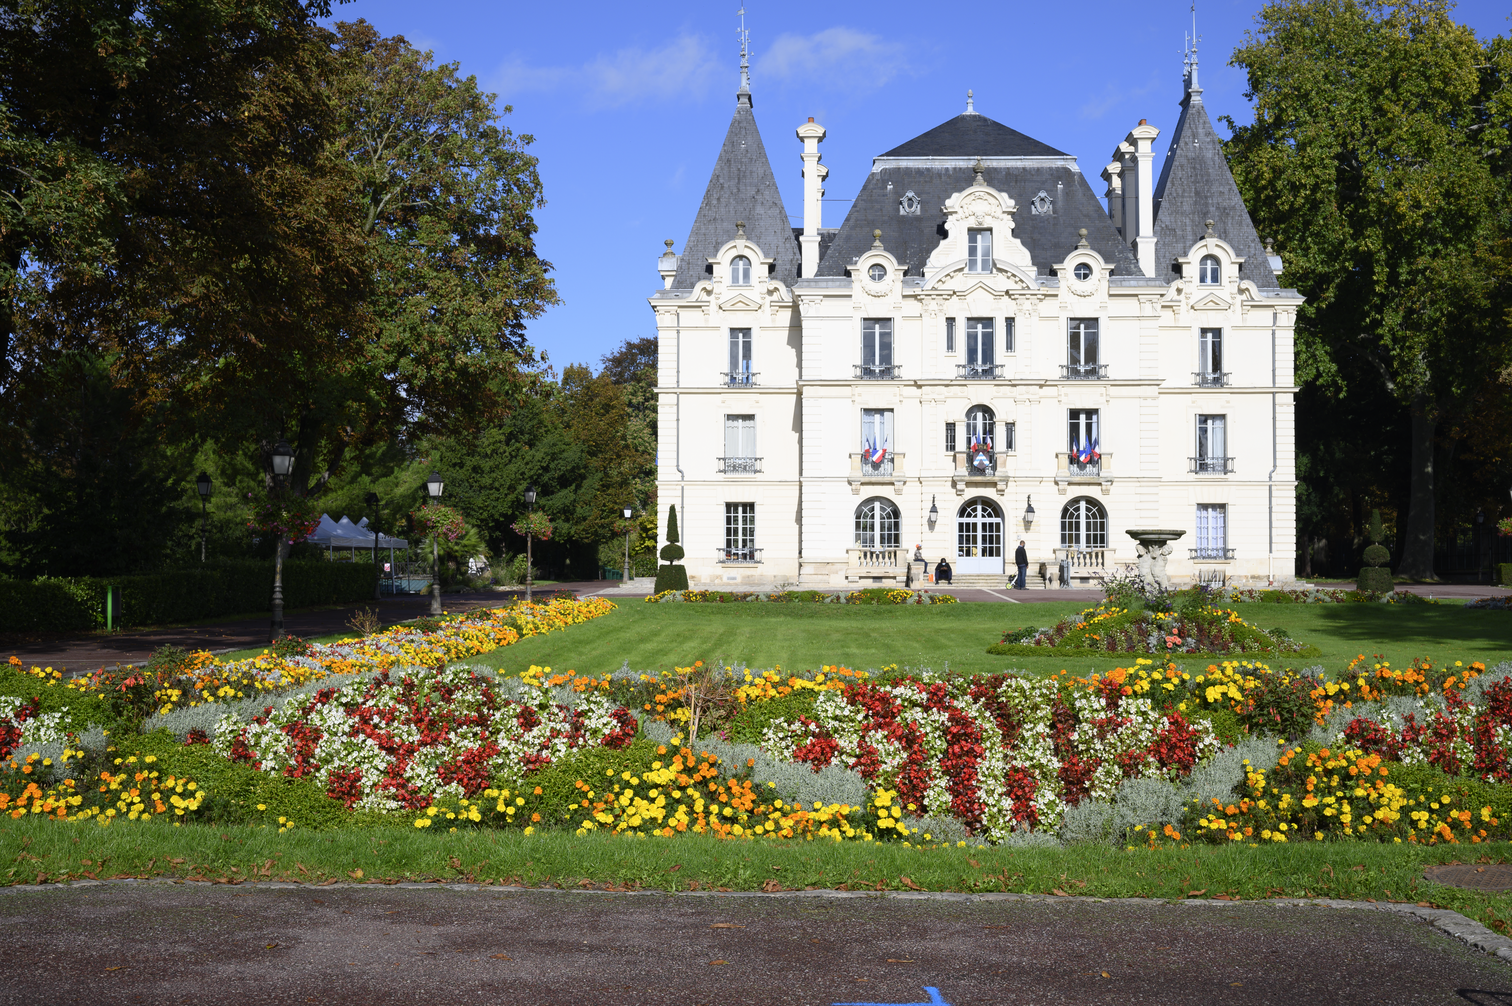
\includegraphics[width=.3\linewidth]{../assets/1512x1006/castle_bg.png}}   &
    \fbox{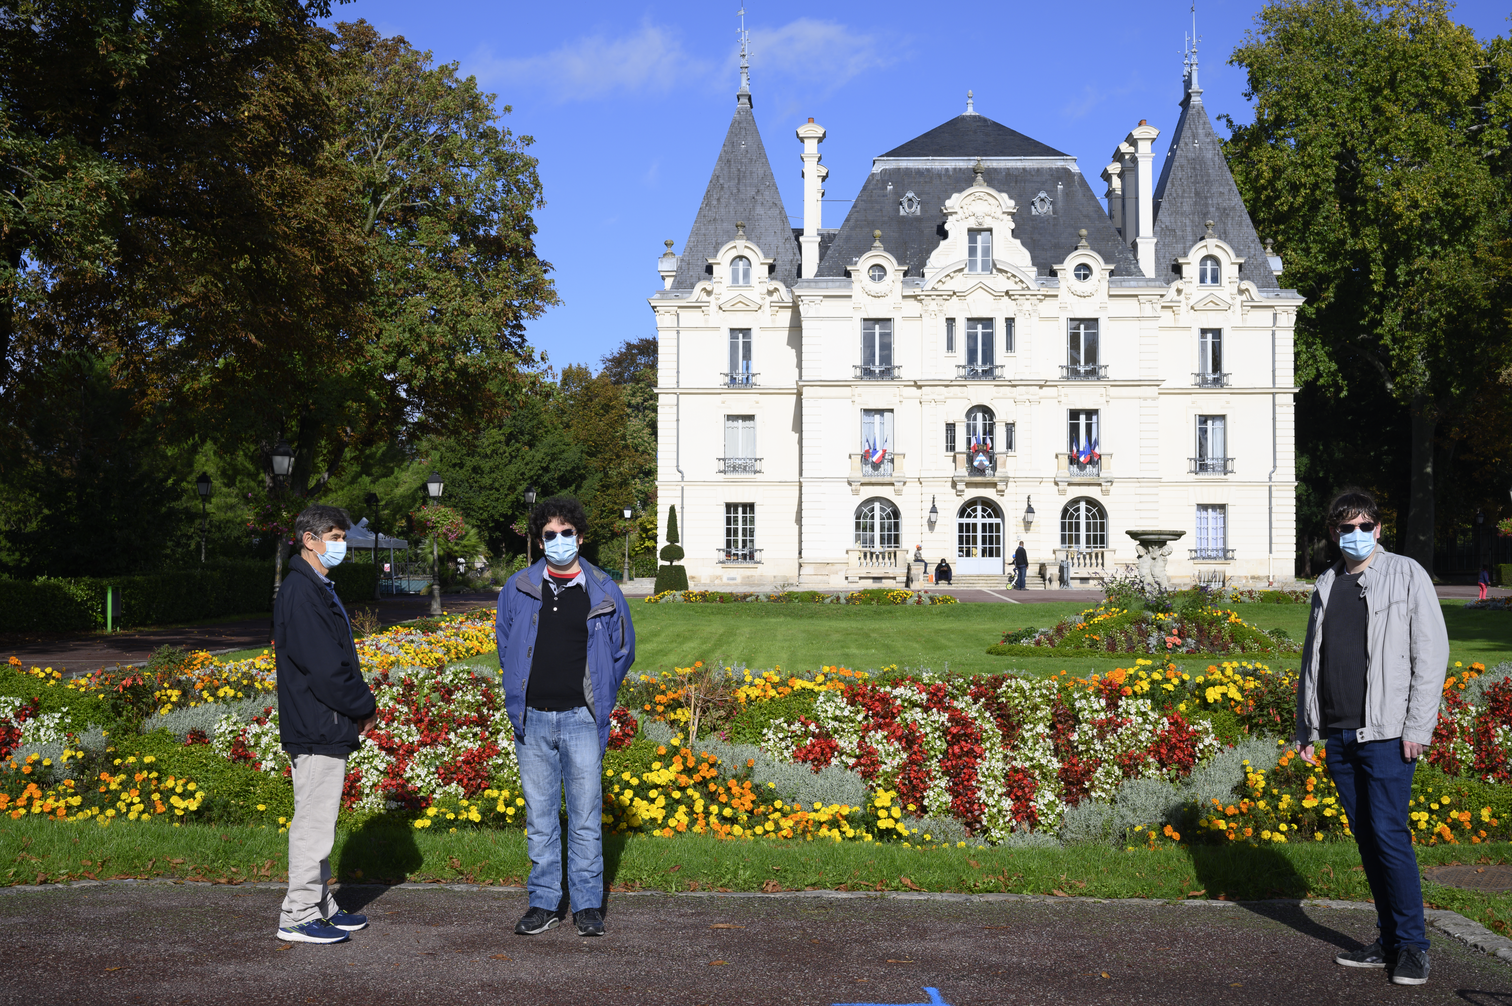
\includegraphics[width=.3\linewidth]{../assets/1512x1006/castle_fg_1.png}} &
    \fbox{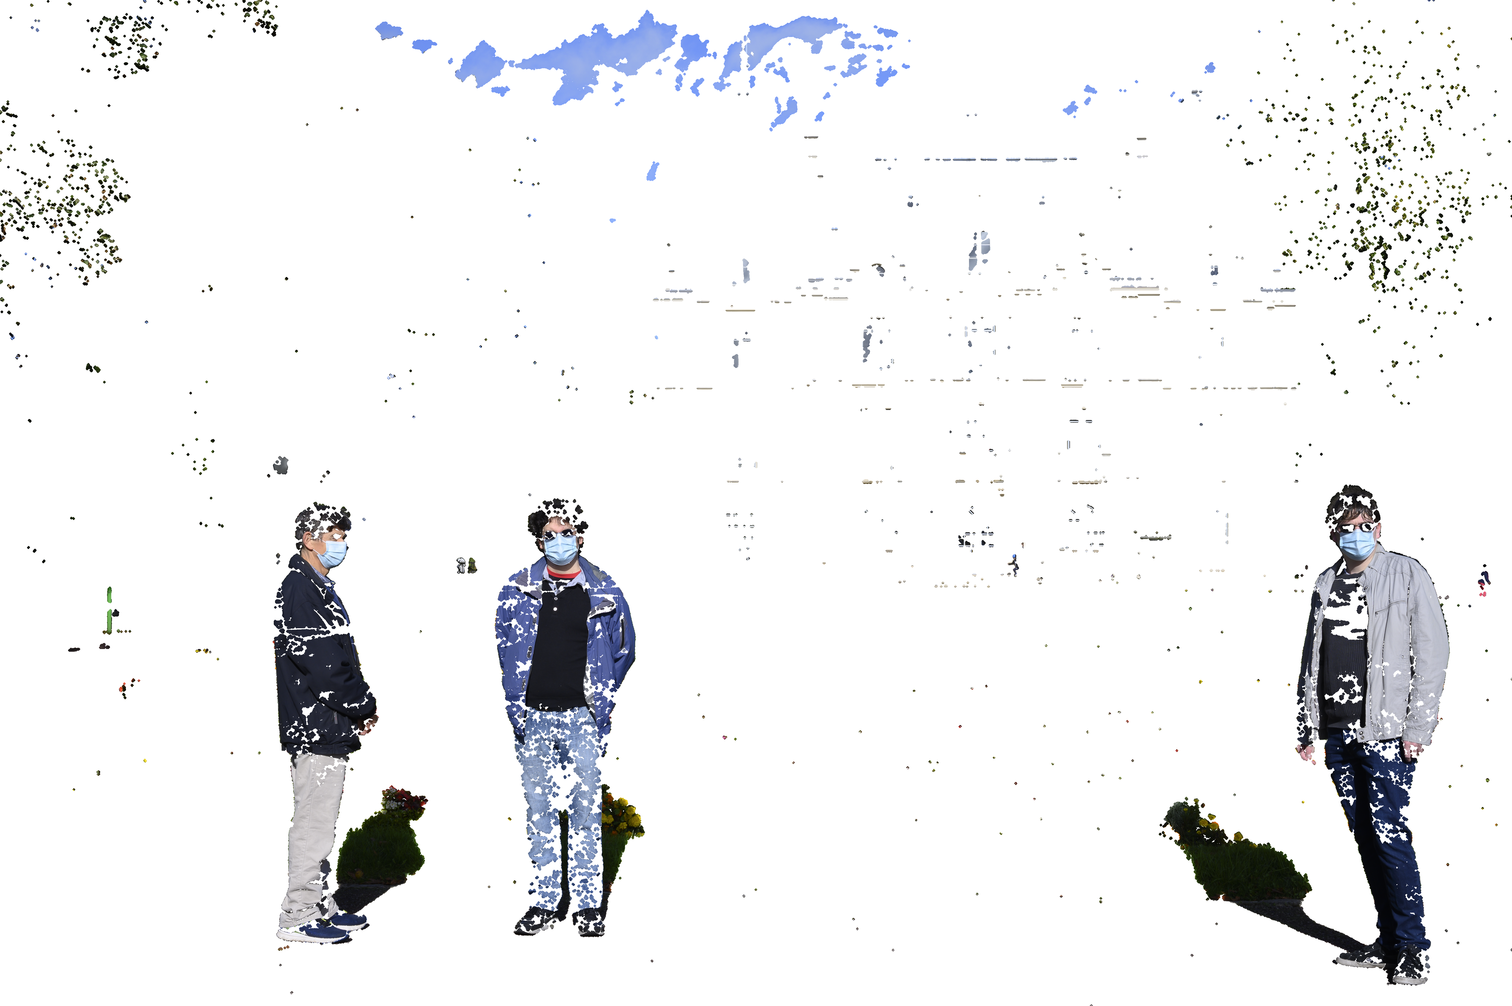
\includegraphics[width=.3\linewidth]{../assets/1512x1006/results_sig1_win5/castle/result_detected_castle_fg_1.png}}
  \end{tabular}

  \caption{Background detection: castle results.}
  \label{fig:bg_sub.castle.restults}
\end{figure}

We have run benchmarks on this set comparing multiple ways of achieving this result, both using Pylene and OpenCV as
well as varying the size and the shape of the structuring element window.The breakdown of these benchmarks are presented
in the figures~\ref{fig:bg_sub.castle.benchmarks} and~\ref{fig:bg_sub.castle.benchmarks.plnonly}.

\begin{figure}[tbh]
  \centering
  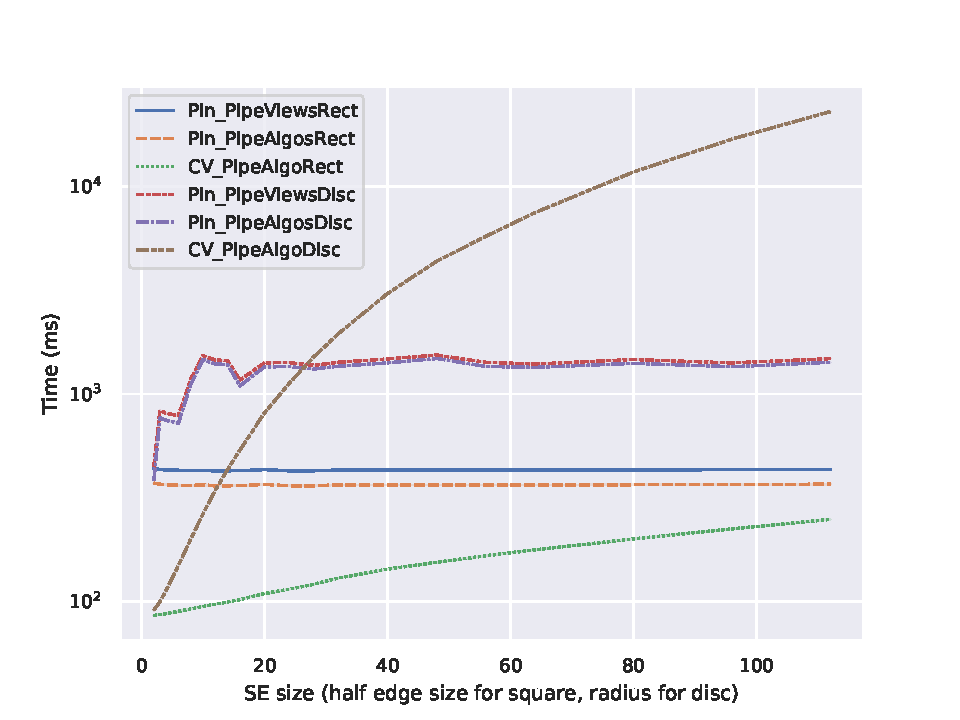
\includegraphics[width=.7\linewidth]{figs/bench/PlnVsOpenCV_bg_sub_0}

  \caption{Background detection: castle benchmark.}
  \label{fig:bg_sub.castle.benchmarks}
\end{figure}

\begin{figure}[tbh]
  \centering
  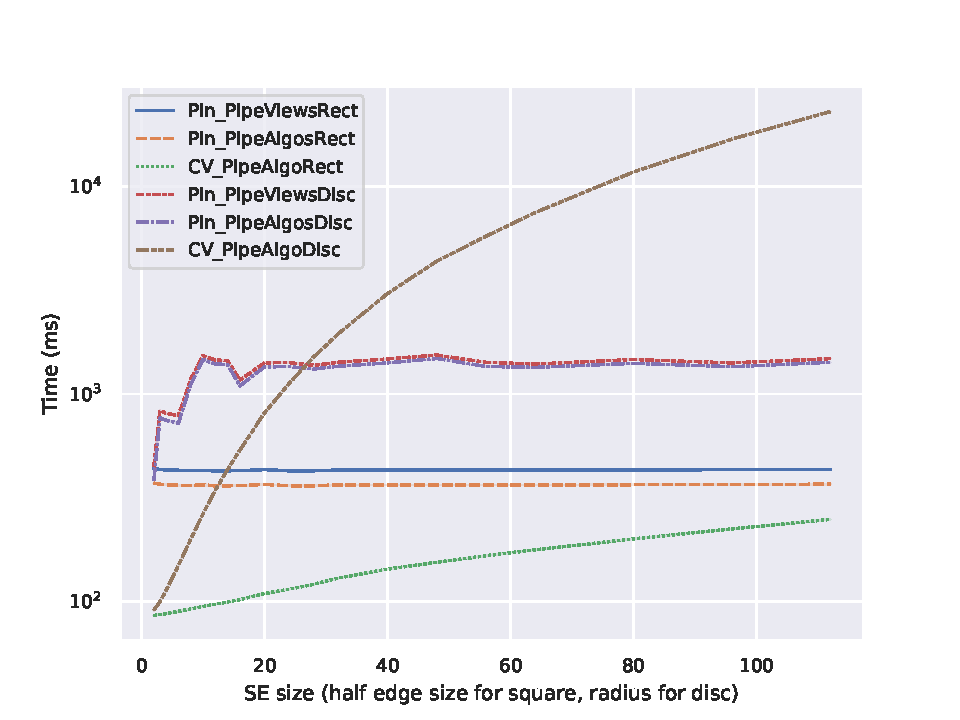
\includegraphics[width=.7\linewidth]{figs/bench/PlnVsOpenCV_bg_sub_0}

  \caption{Background detection: castle benchmark, Pylene only.}
  \label{fig:bg_sub.castle.benchmarks.plnonly}
\end{figure}

\paragraph{Set \#2: garden} We have also run the algorithm on another another original set of images presented in
figure~\ref{fig:bg_sub.garden.restults}.

\begin{figure}[tbh]
  \centering
  \begin{tabular}{cccc}
    Background
                                                                                     & Candidate & Result                     \\[5pt]
    \fbox{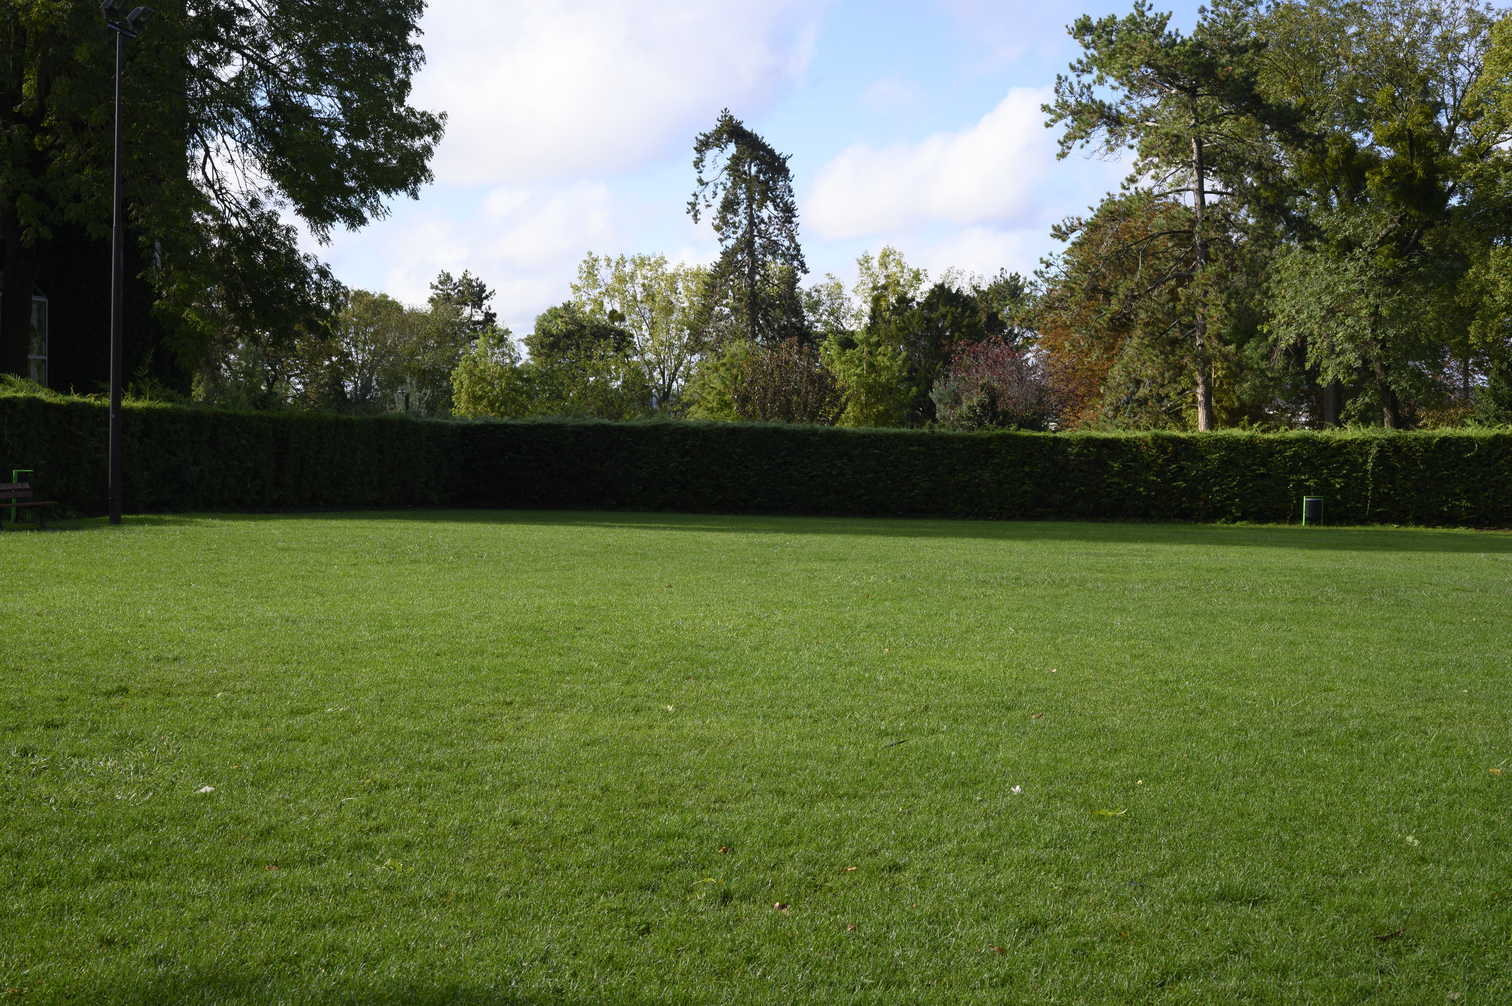
\includegraphics[width=.3\linewidth]{../assets/1512x1006/garden_bg.png}}   &
    \fbox{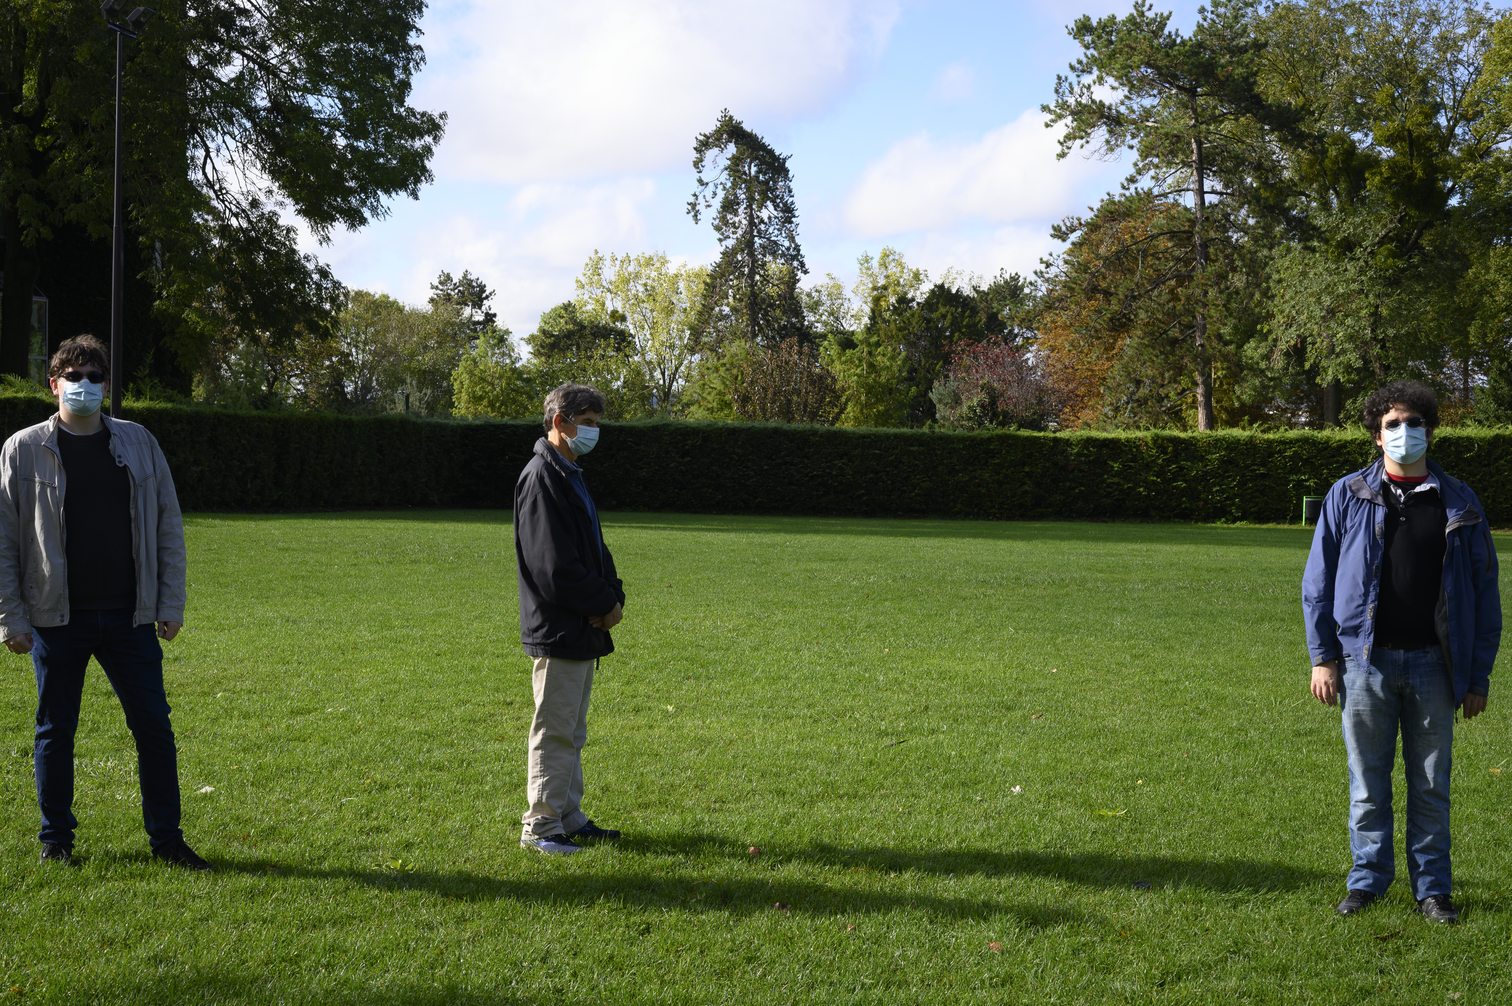
\includegraphics[width=.3\linewidth]{../assets/1512x1006/garden_fg_1.png}} &
    \fbox{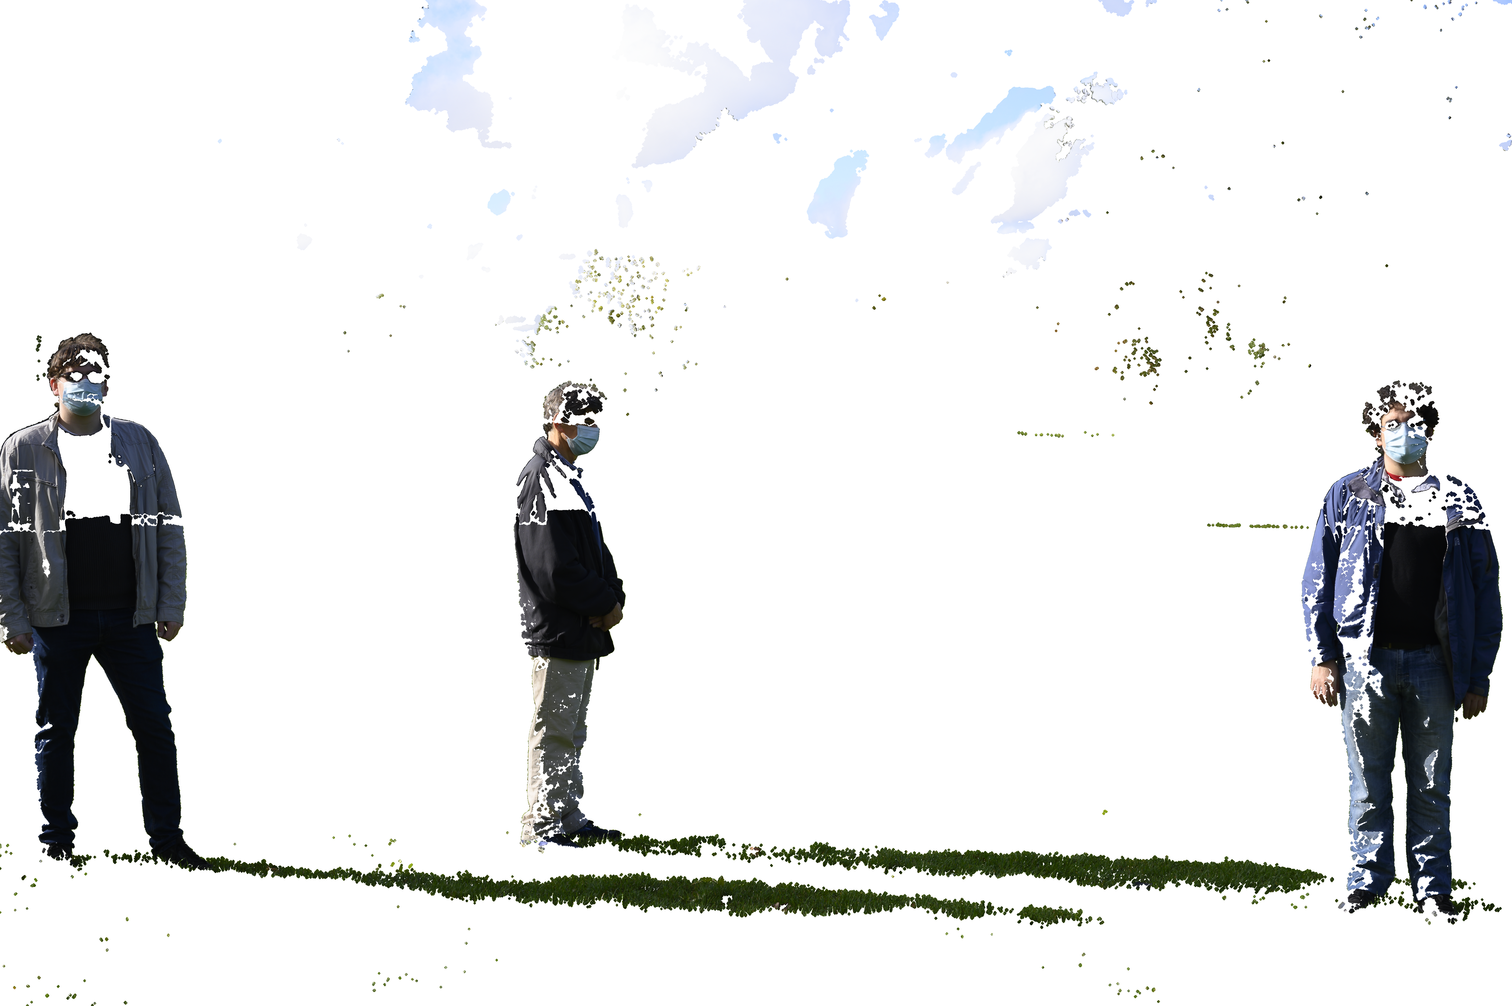
\includegraphics[width=.3\linewidth]{../assets/1512x1006/results_sig1_win5/garden/result_detected_garden_fg_1.png}} \\[5pt]
    \fbox{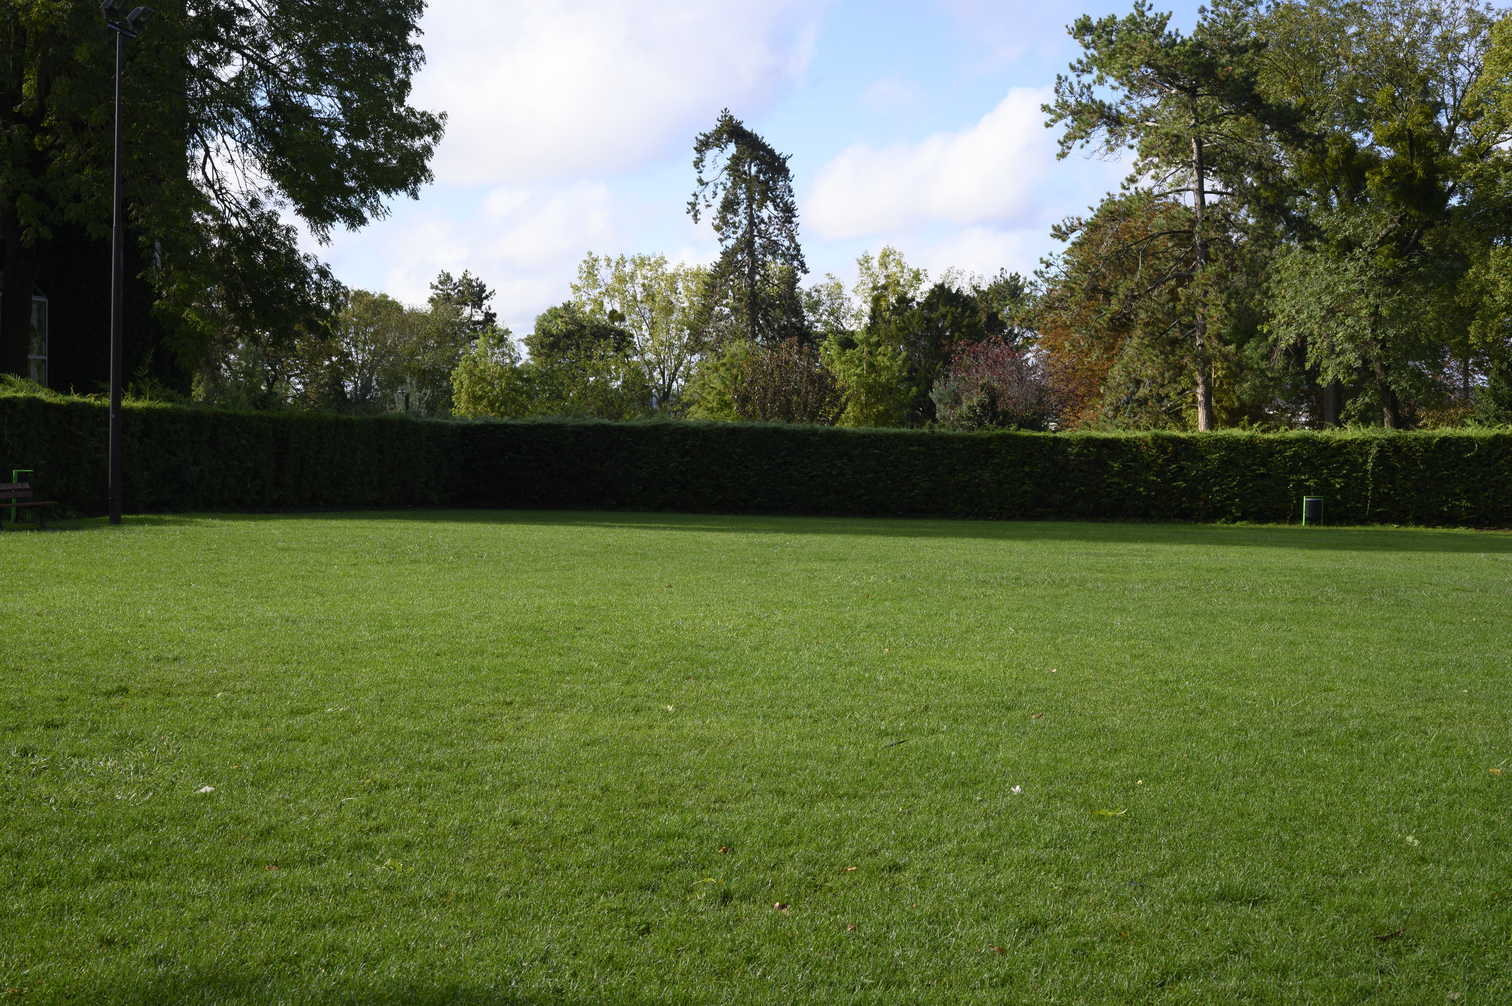
\includegraphics[width=.3\linewidth]{../assets/1512x1006/garden_bg.png}}   &
    \fbox{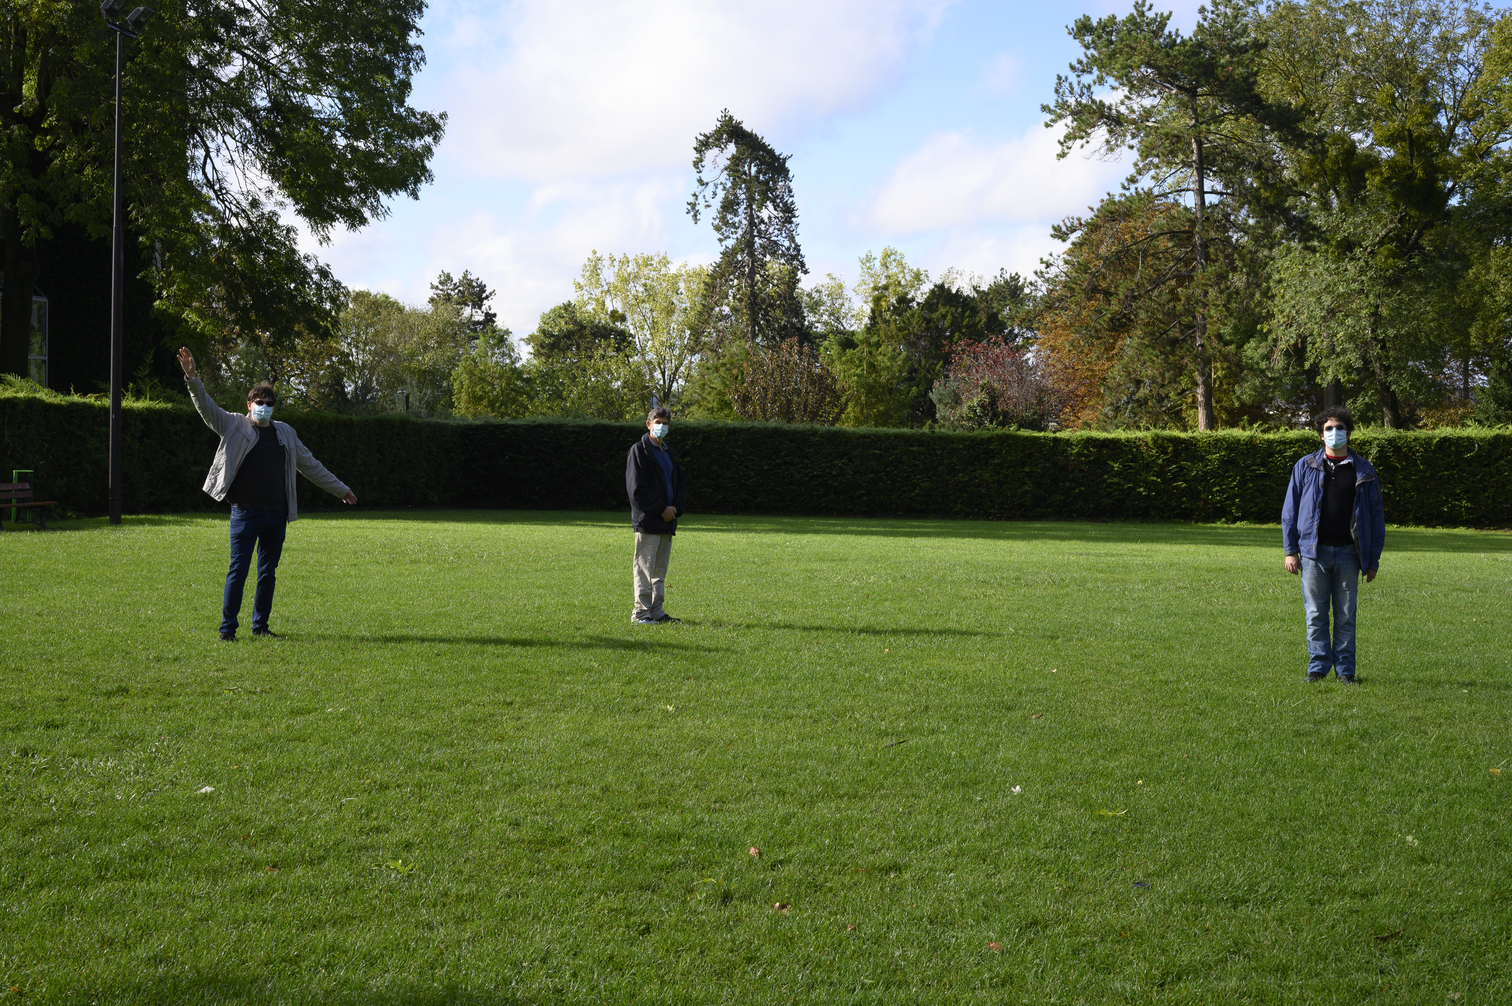
\includegraphics[width=.3\linewidth]{../assets/1512x1006/garden_fg_2.png}} &
    \fbox{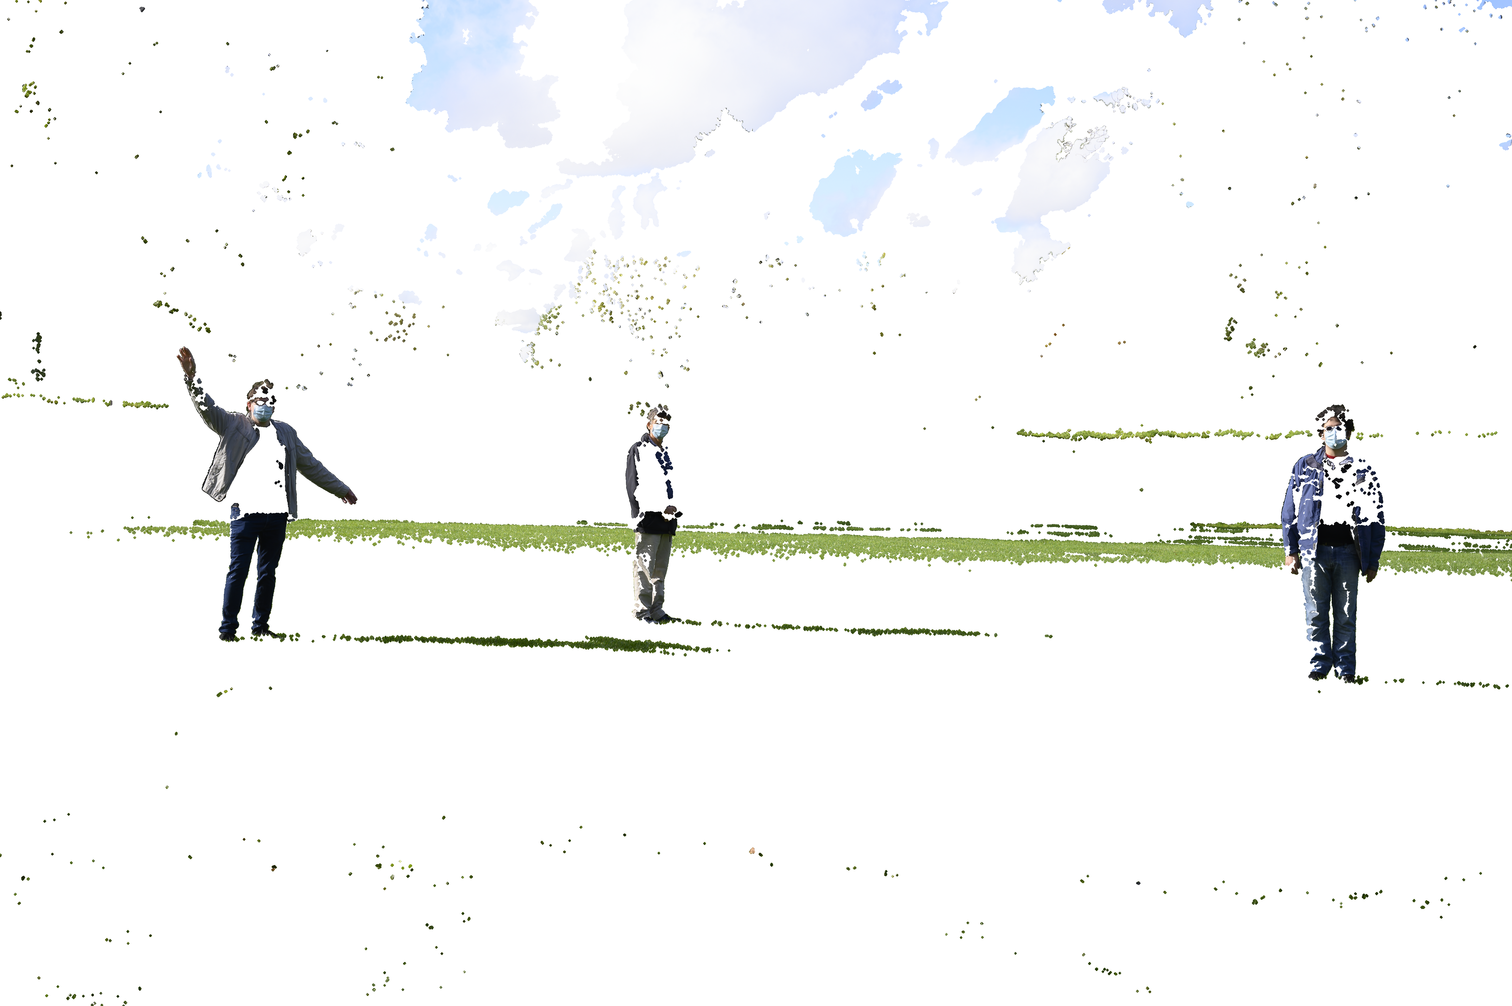
\includegraphics[width=.3\linewidth]{../assets/1512x1006/results_sig1_win5/garden/result_detected_garden_fg_2.png}} \\[5pt]
    \fbox{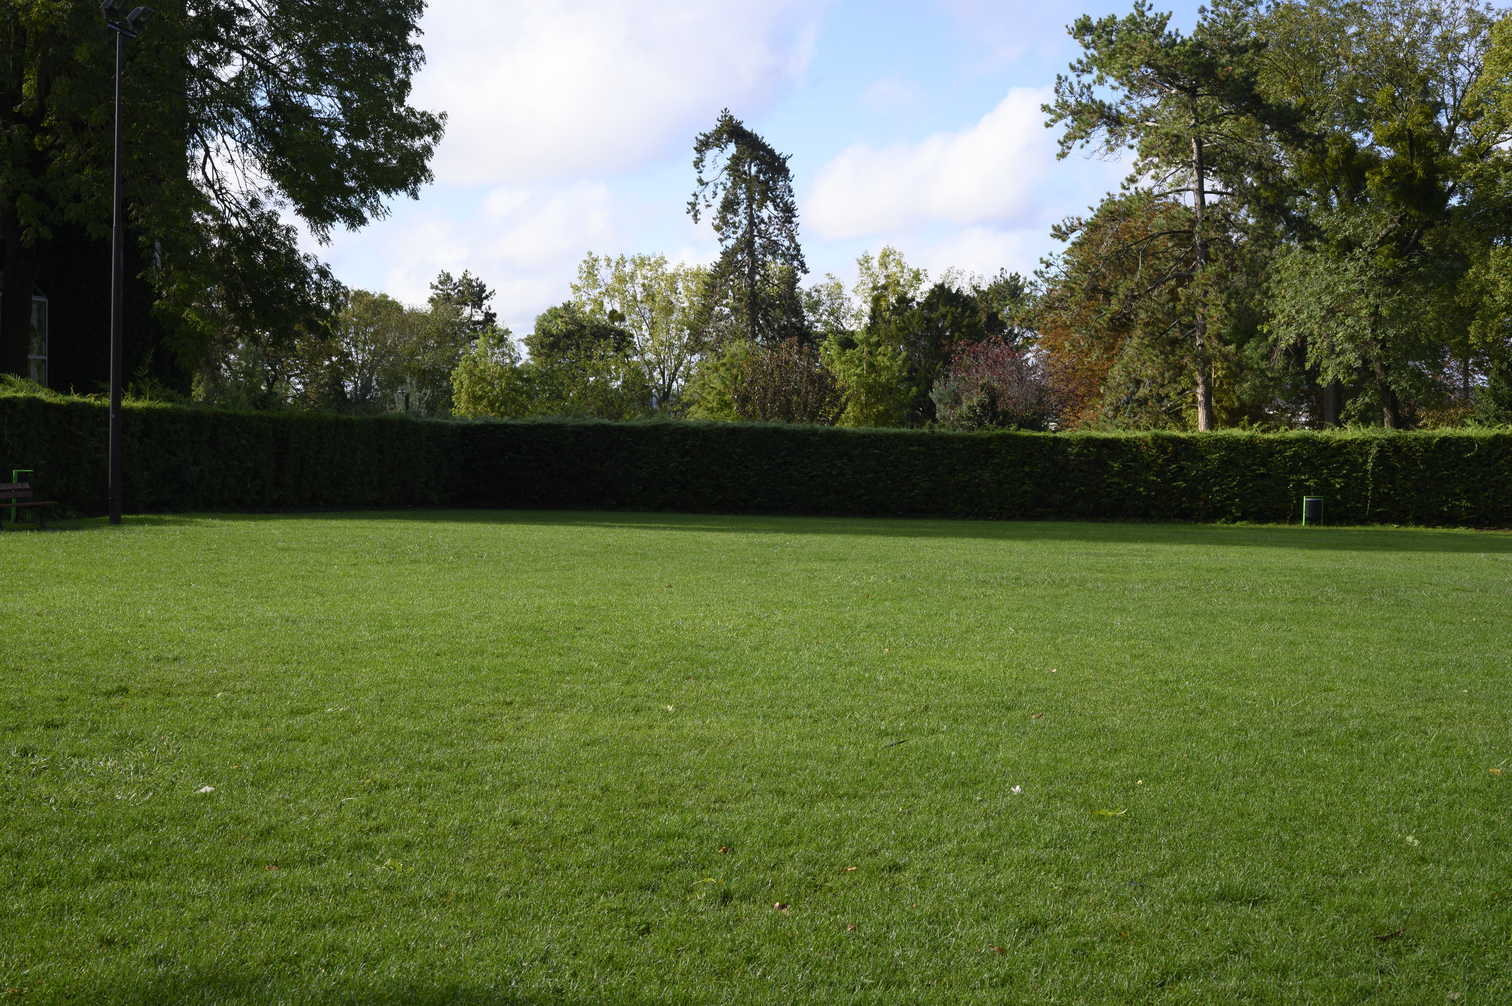
\includegraphics[width=.3\linewidth]{../assets/1512x1006/garden_bg.png}}   &
    \fbox{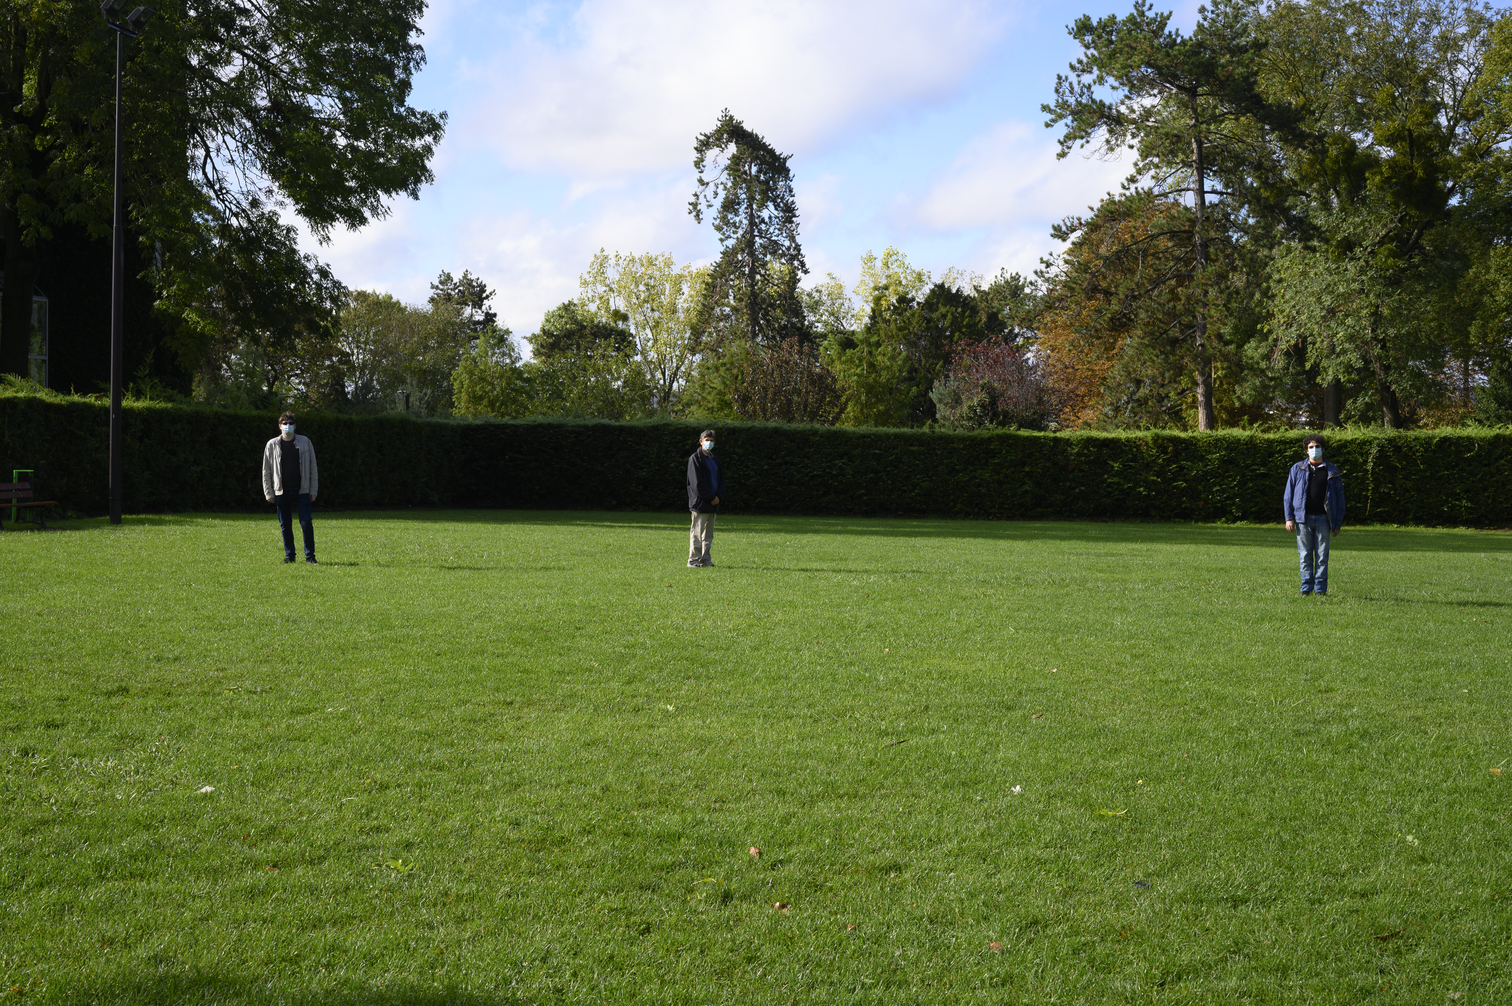
\includegraphics[width=.3\linewidth]{../assets/1512x1006/garden_fg_3.png}} &
    \fbox{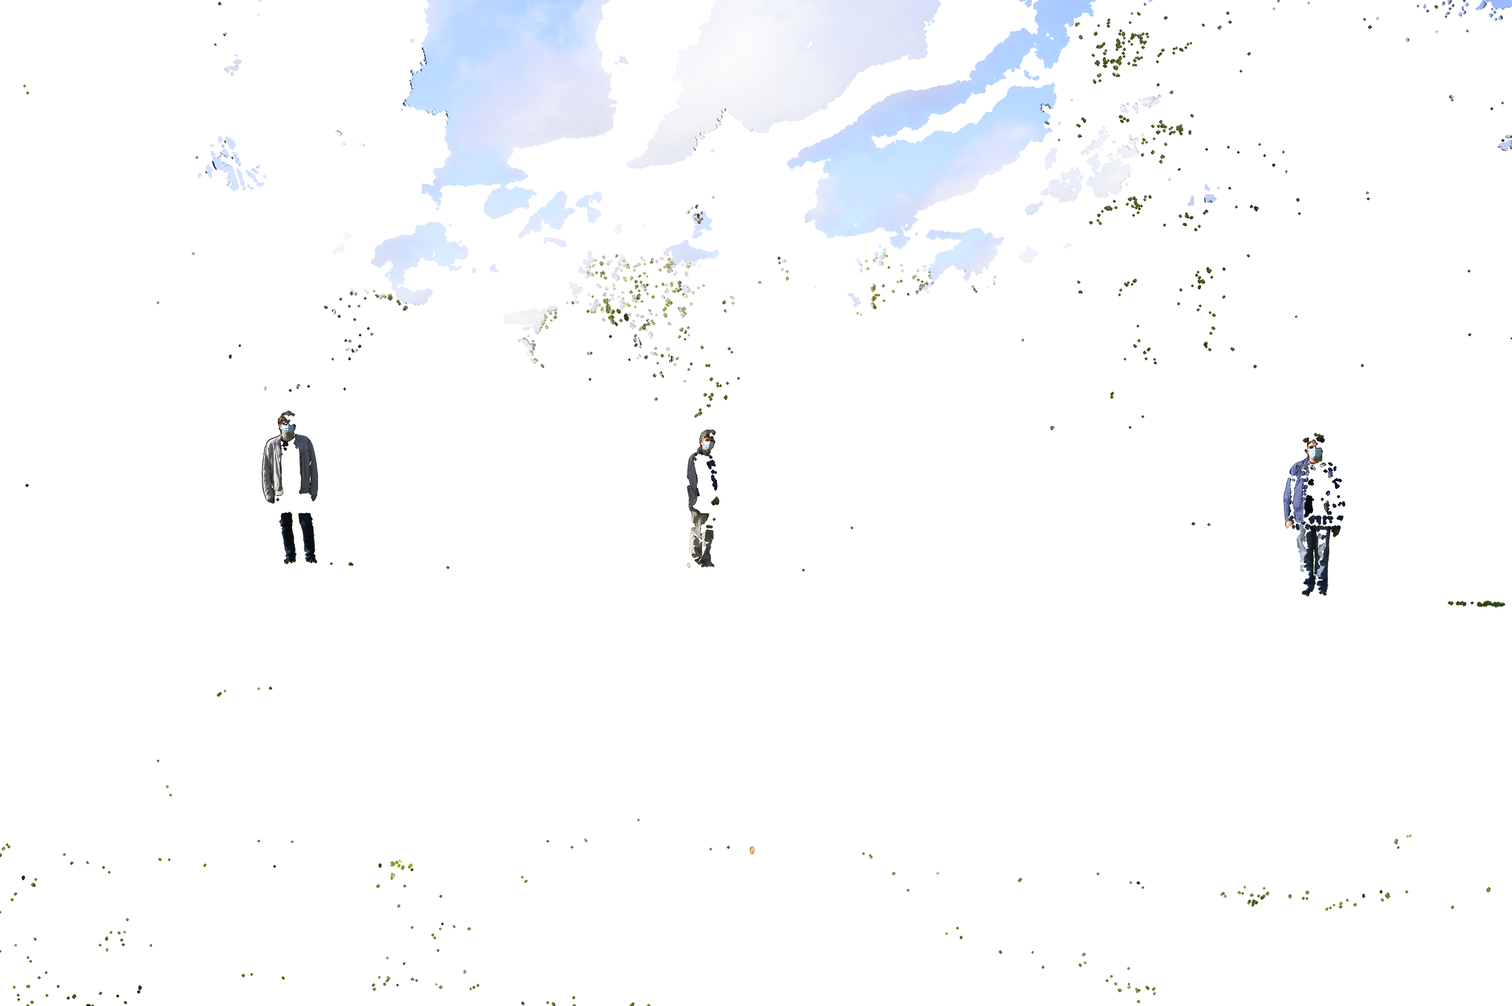
\includegraphics[width=.3\linewidth]{../assets/1512x1006/results_sig1_win5/garden/result_detected_garden_fg_3.png}} \\[5pt]
    \fbox{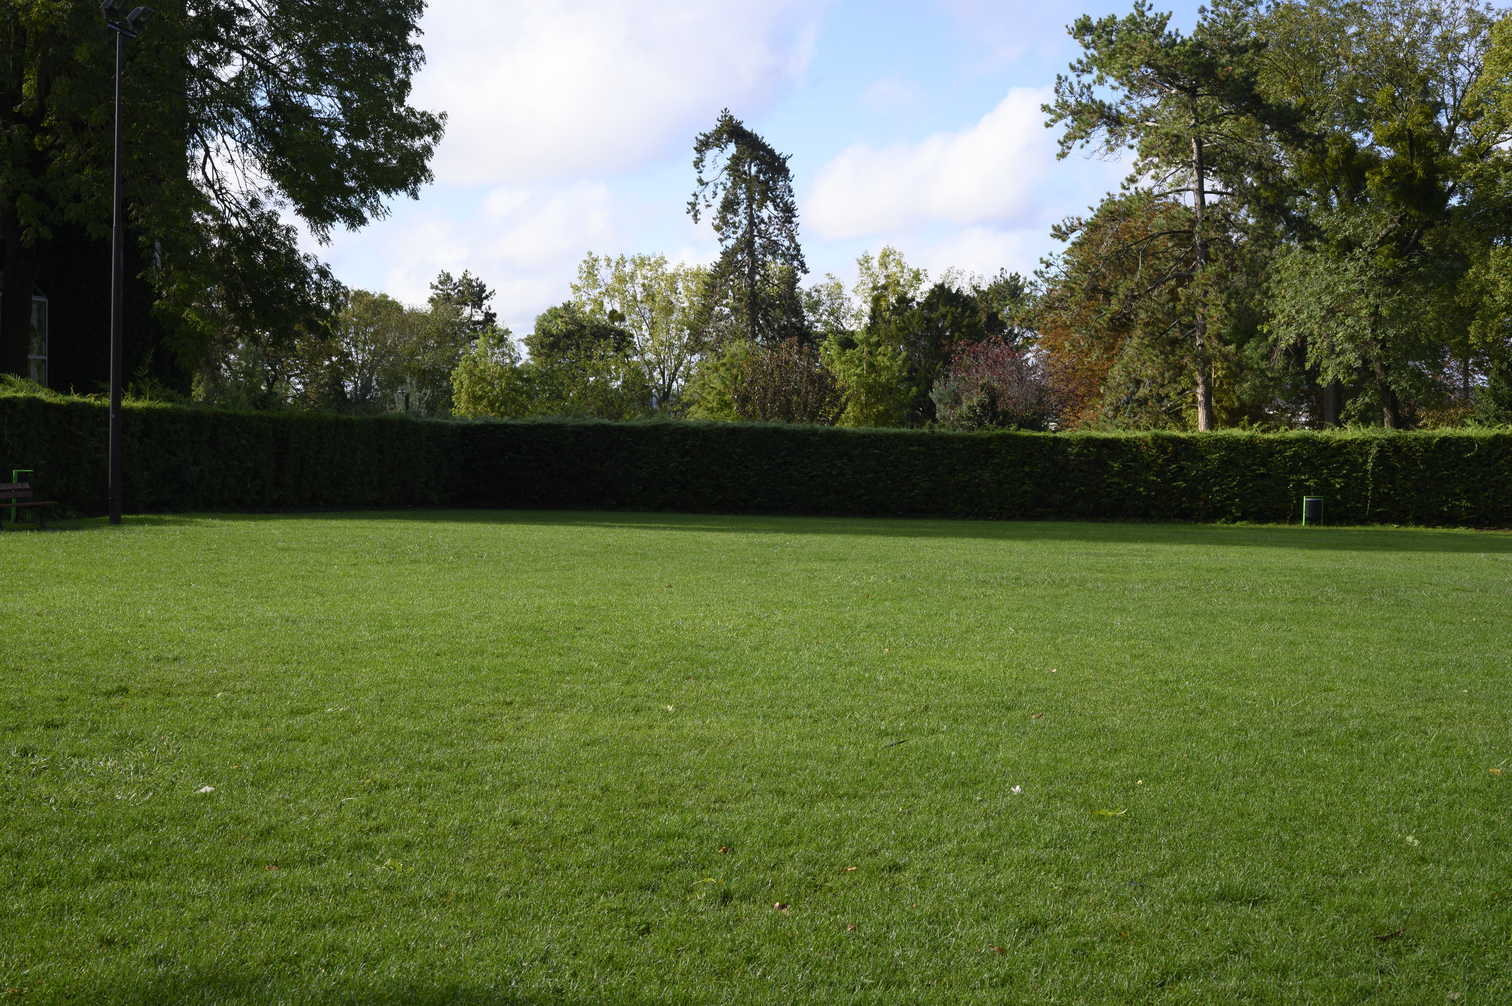
\includegraphics[width=.3\linewidth]{../assets/1512x1006/garden_bg.png}}   &
    \fbox{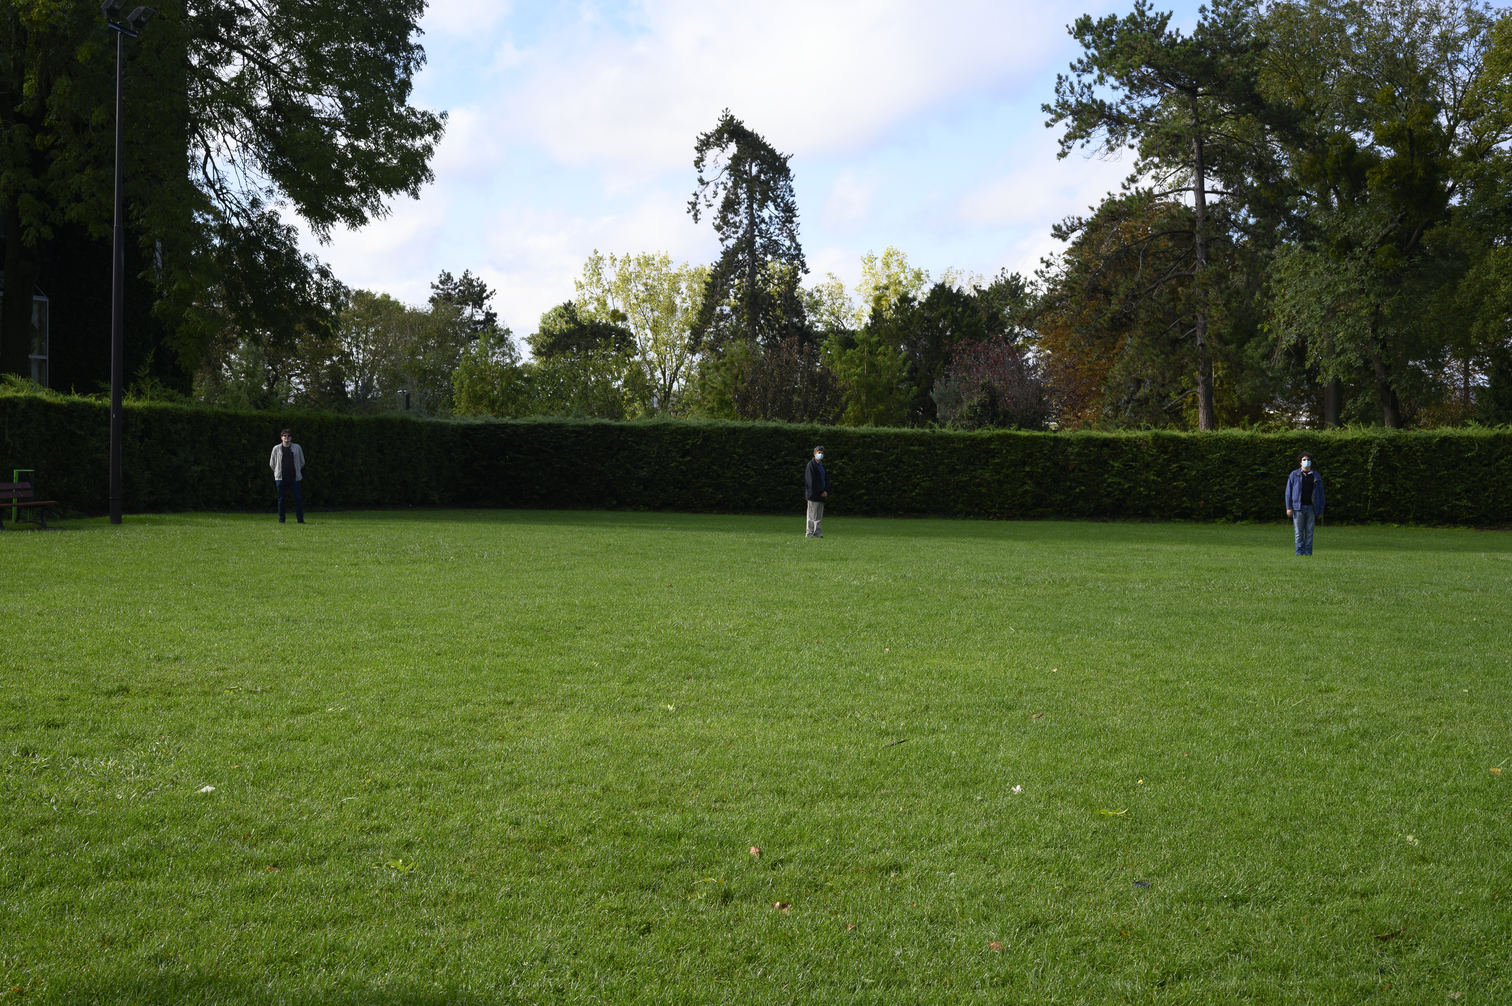
\includegraphics[width=.3\linewidth]{../assets/1512x1006/garden_fg_4.png}} &
    \fbox{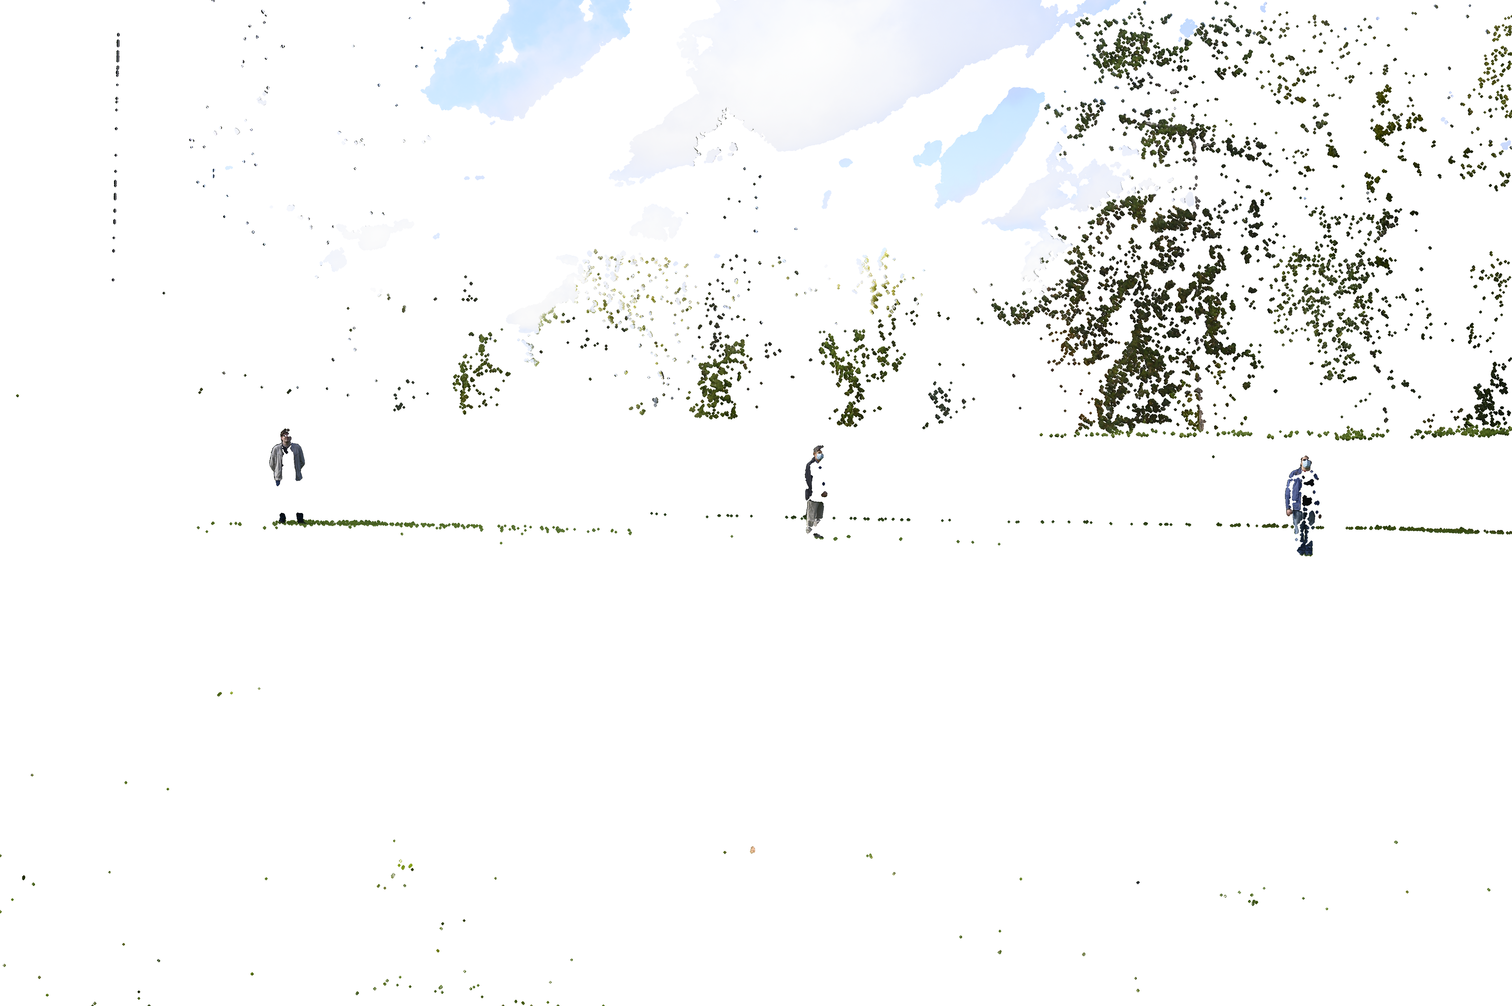
\includegraphics[width=.3\linewidth]{../assets/1512x1006/results_sig1_win5/garden/result_detected_garden_fg_4.png}} \\[5pt]
    \fbox{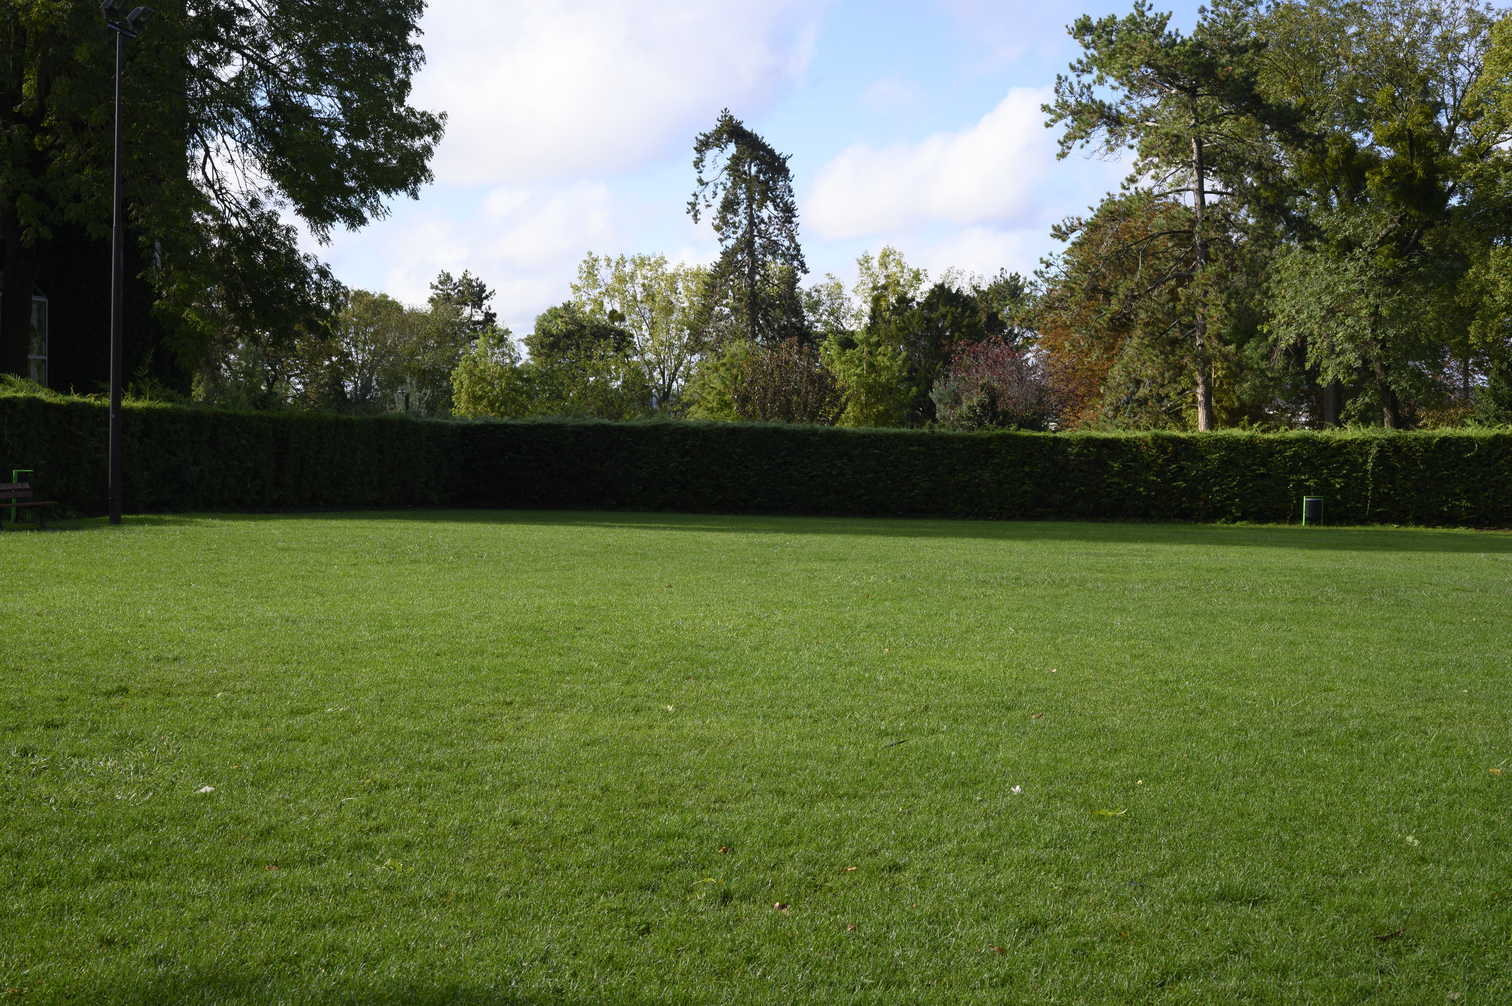
\includegraphics[width=.3\linewidth]{../assets/1512x1006/garden_bg.png}}   &
    \fbox{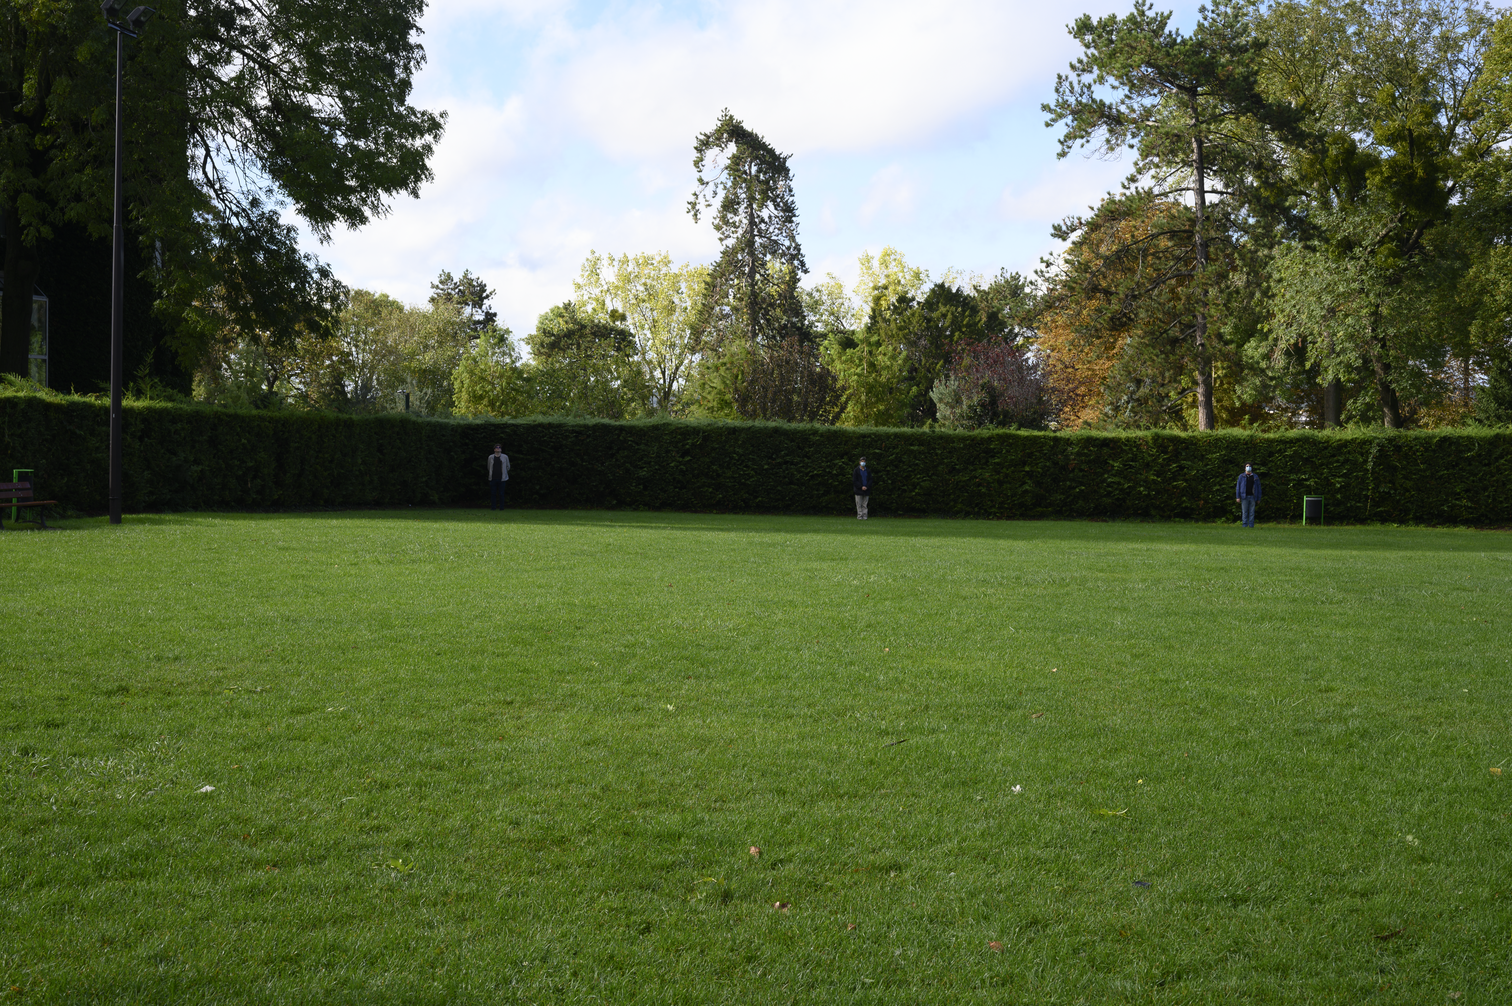
\includegraphics[width=.3\linewidth]{../assets/1512x1006/garden_fg_5.png}} &
    \fbox{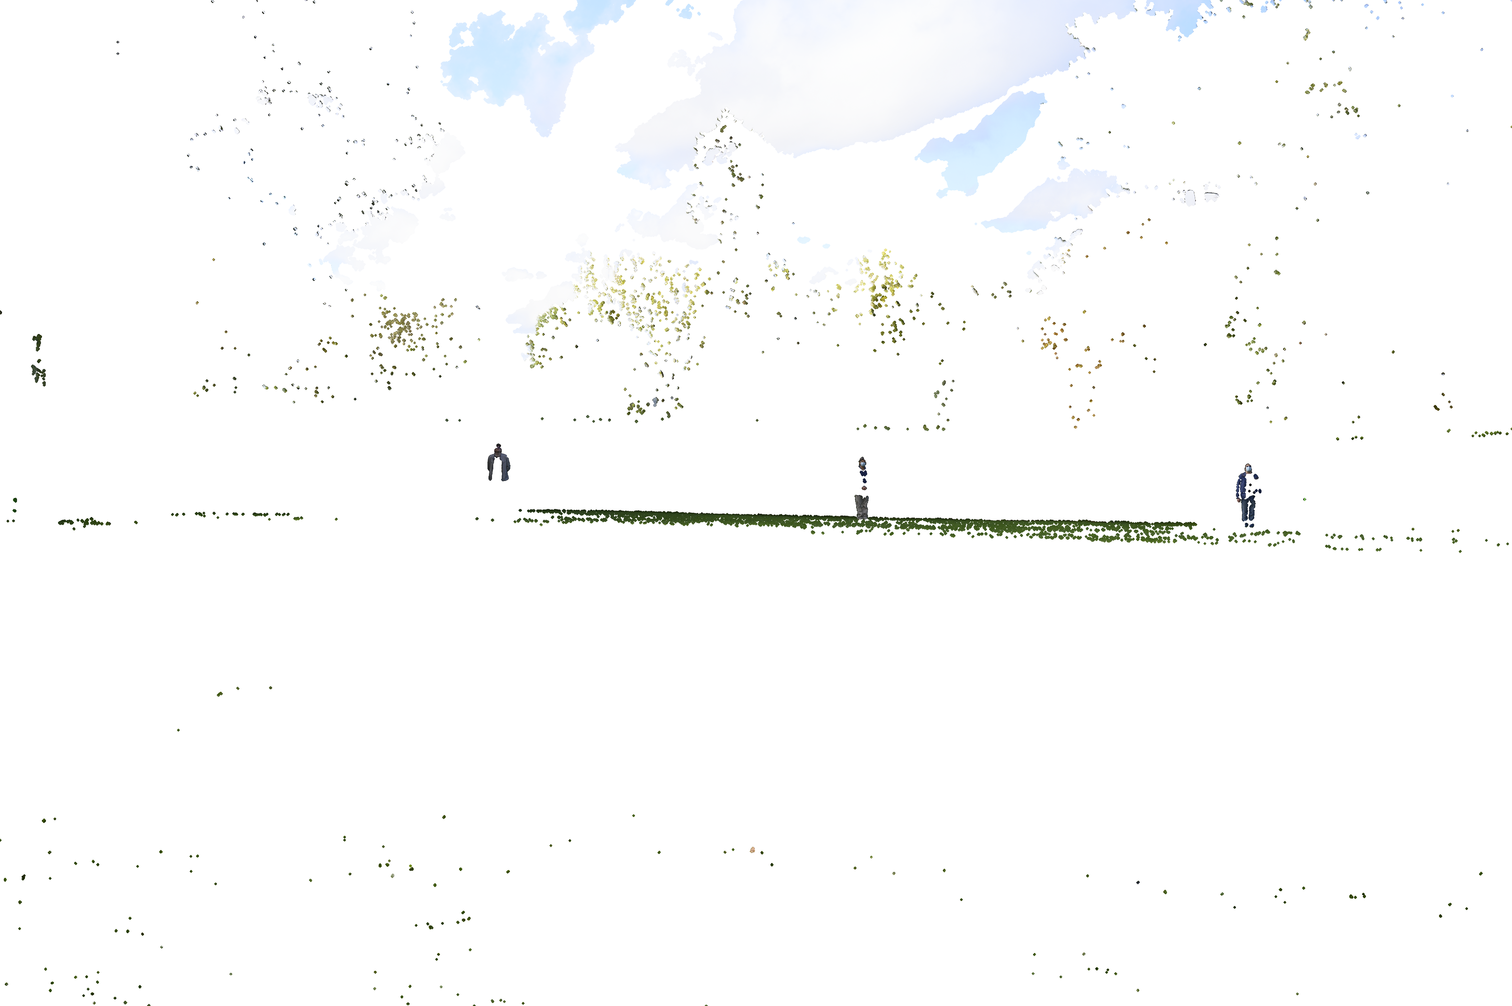
\includegraphics[width=.3\linewidth]{../assets/1512x1006/results_sig1_win5/garden/result_detected_garden_fg_5.png}}
  \end{tabular}

  \caption{Background detection: garden results.}
  \label{fig:bg_sub.garden.restults}
\end{figure}

The breakdown of the benchmarks corresponding to this original set is presented in the
figures~\ref{fig:bg_sub.garden.benchmarks}.

\begin{figure}[tbh]
  \centering
  \begin{tabular}{cccc}
    Result                                                                                                                    & Benchmark & Benchmark Pln only \\[5pt]
    \fbox{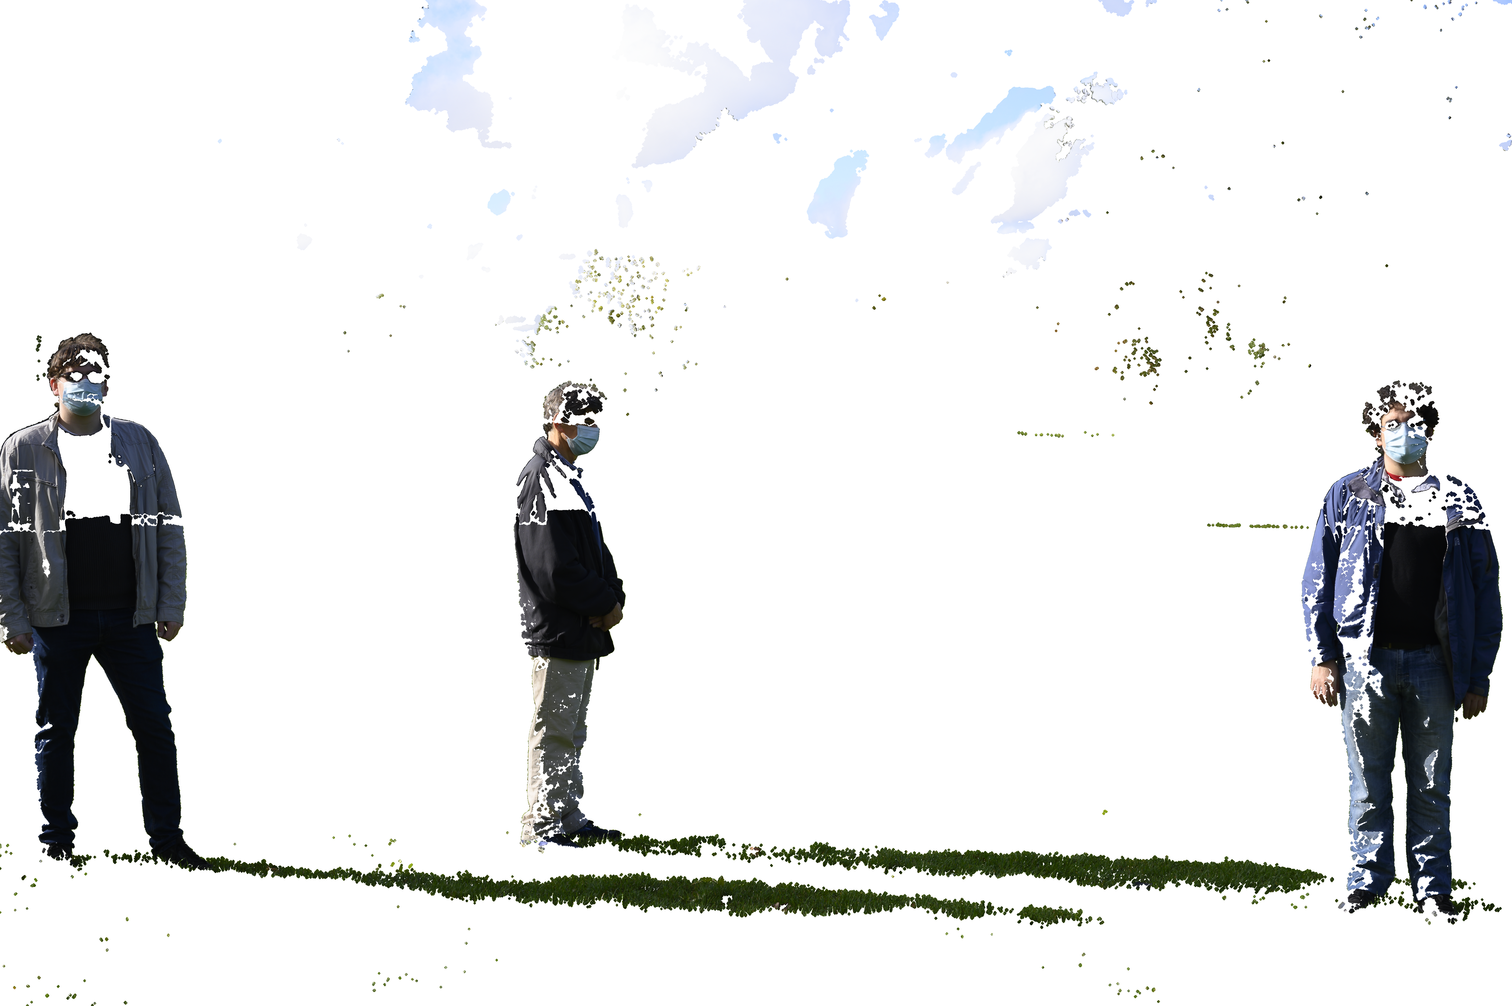
\includegraphics[width=.3\linewidth]{../assets/1512x1006/results_sig1_win5/garden/result_detected_garden_fg_1.png}} &
    \fbox{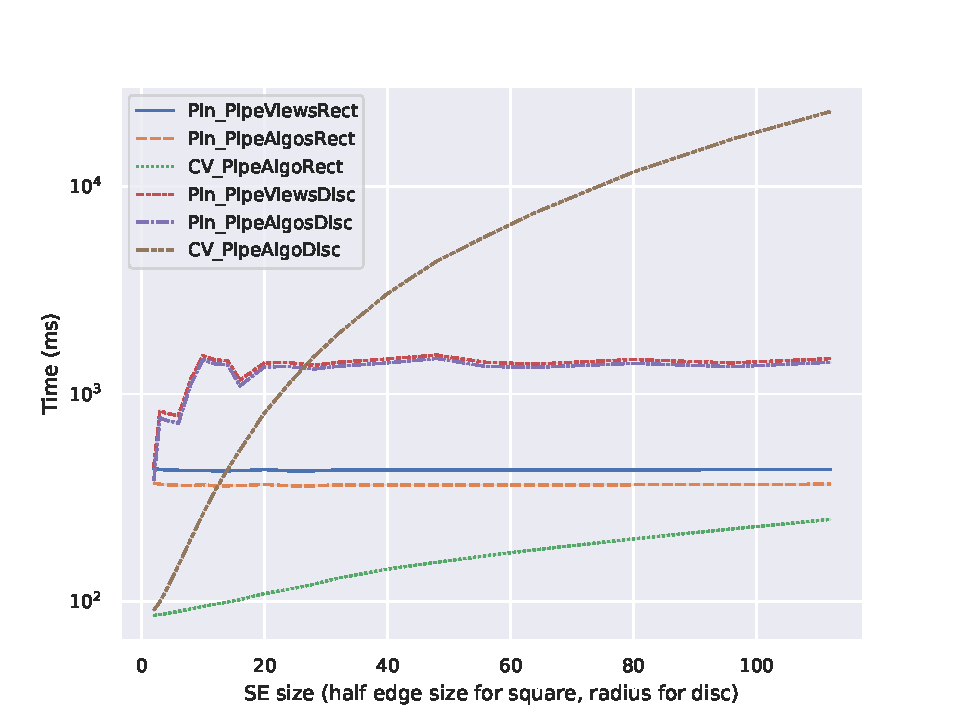
\includegraphics[width=.3\linewidth]{figs/bench/PlnVsOpenCV_bg_sub_1.pdf}}                                          &
    \fbox{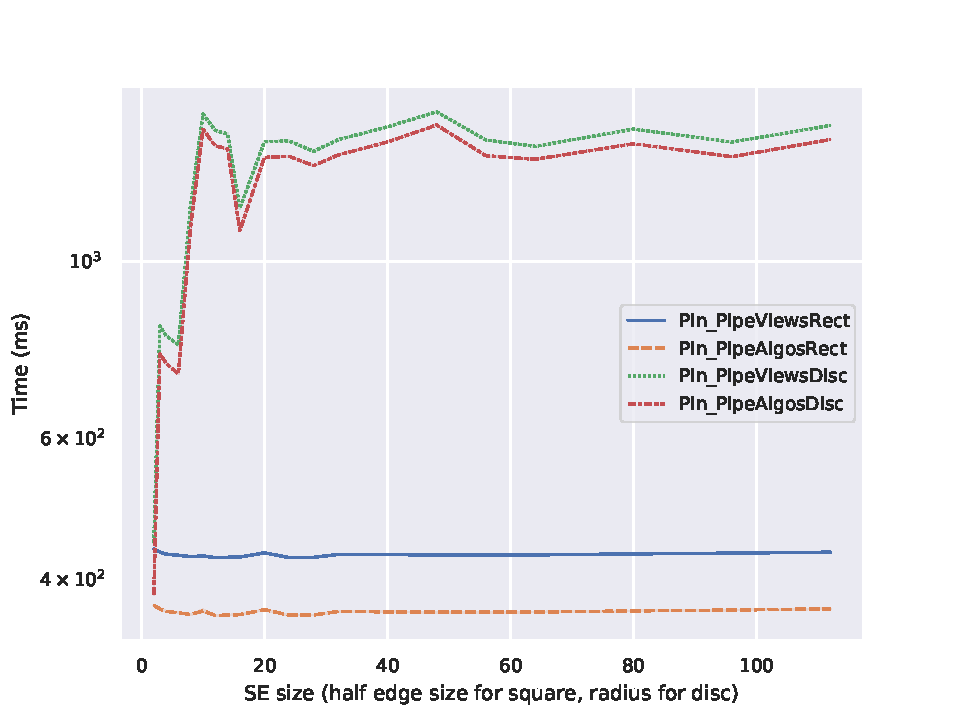
\includegraphics[width=.3\linewidth]{figs/bench/PlnVsOpenCV_bg_sub_pln_1.pdf}}                                                                       \\[5pt]
    \fbox{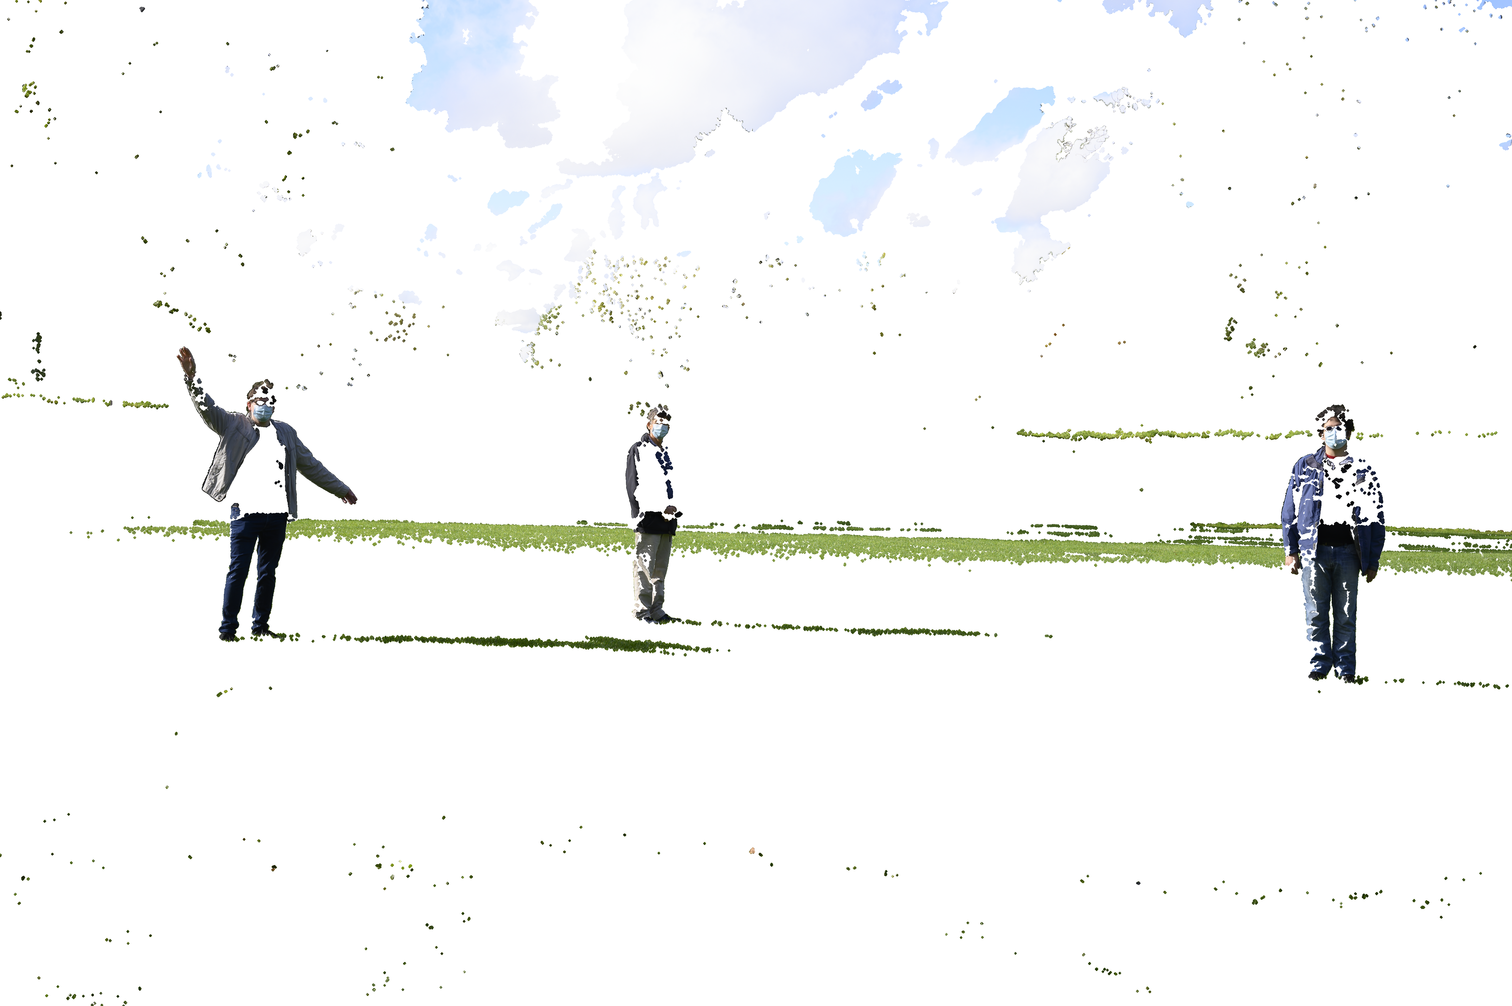
\includegraphics[width=.3\linewidth]{../assets/1512x1006/results_sig1_win5/garden/result_detected_garden_fg_2.png}} &
    \fbox{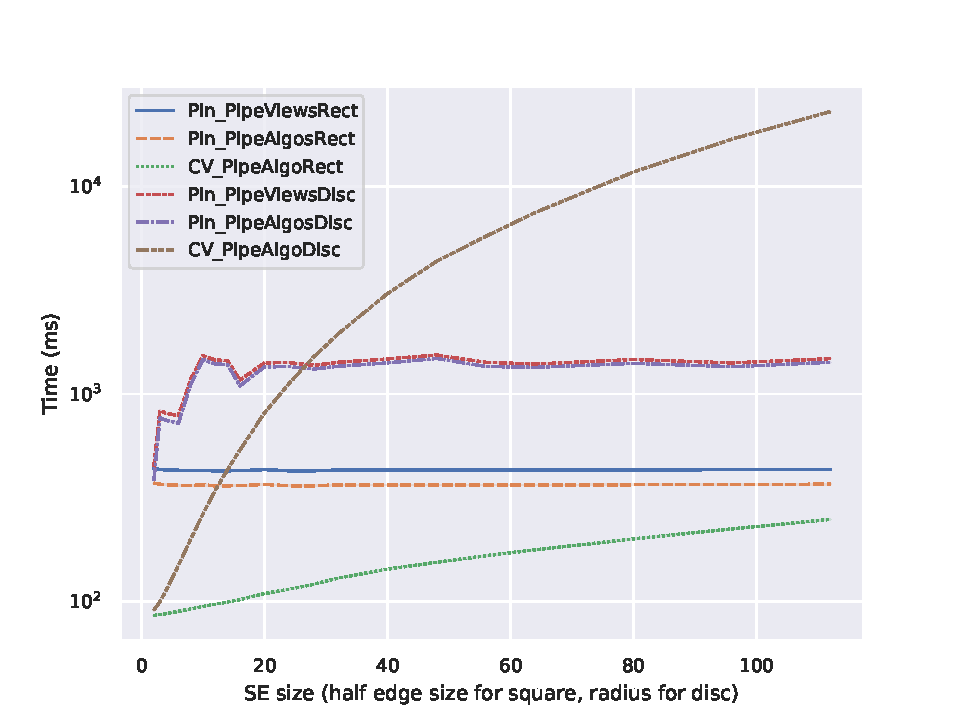
\includegraphics[width=.3\linewidth]{figs/bench/PlnVsOpenCV_bg_sub_2.pdf}}                                          &
    \fbox{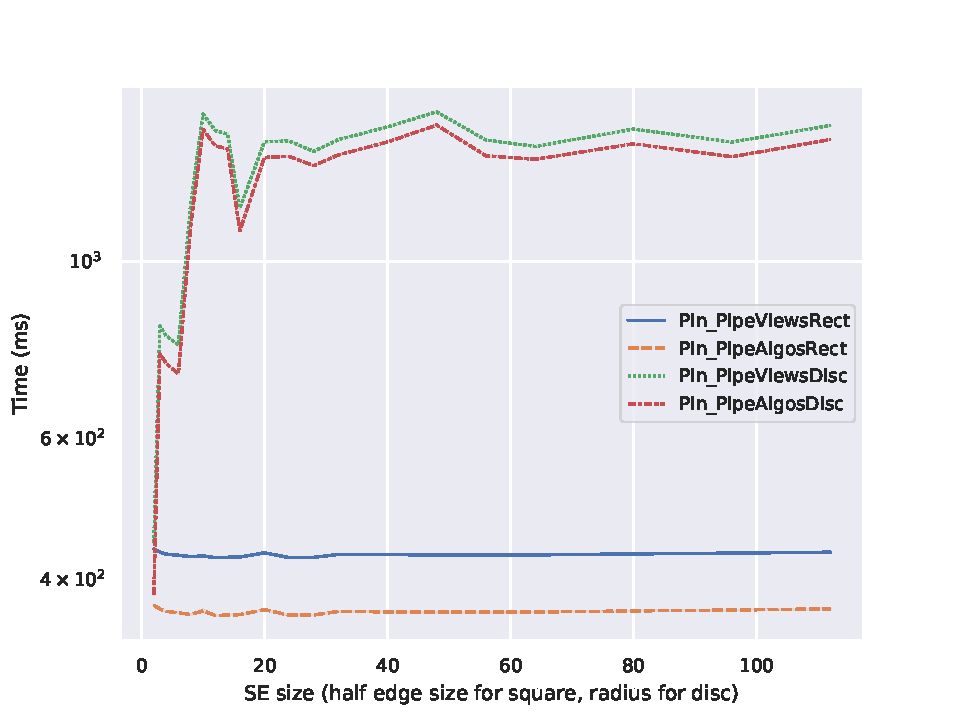
\includegraphics[width=.3\linewidth]{figs/bench/PlnVsOpenCV_bg_sub_pln_2.pdf}}                                                                       \\[5pt]
    \fbox{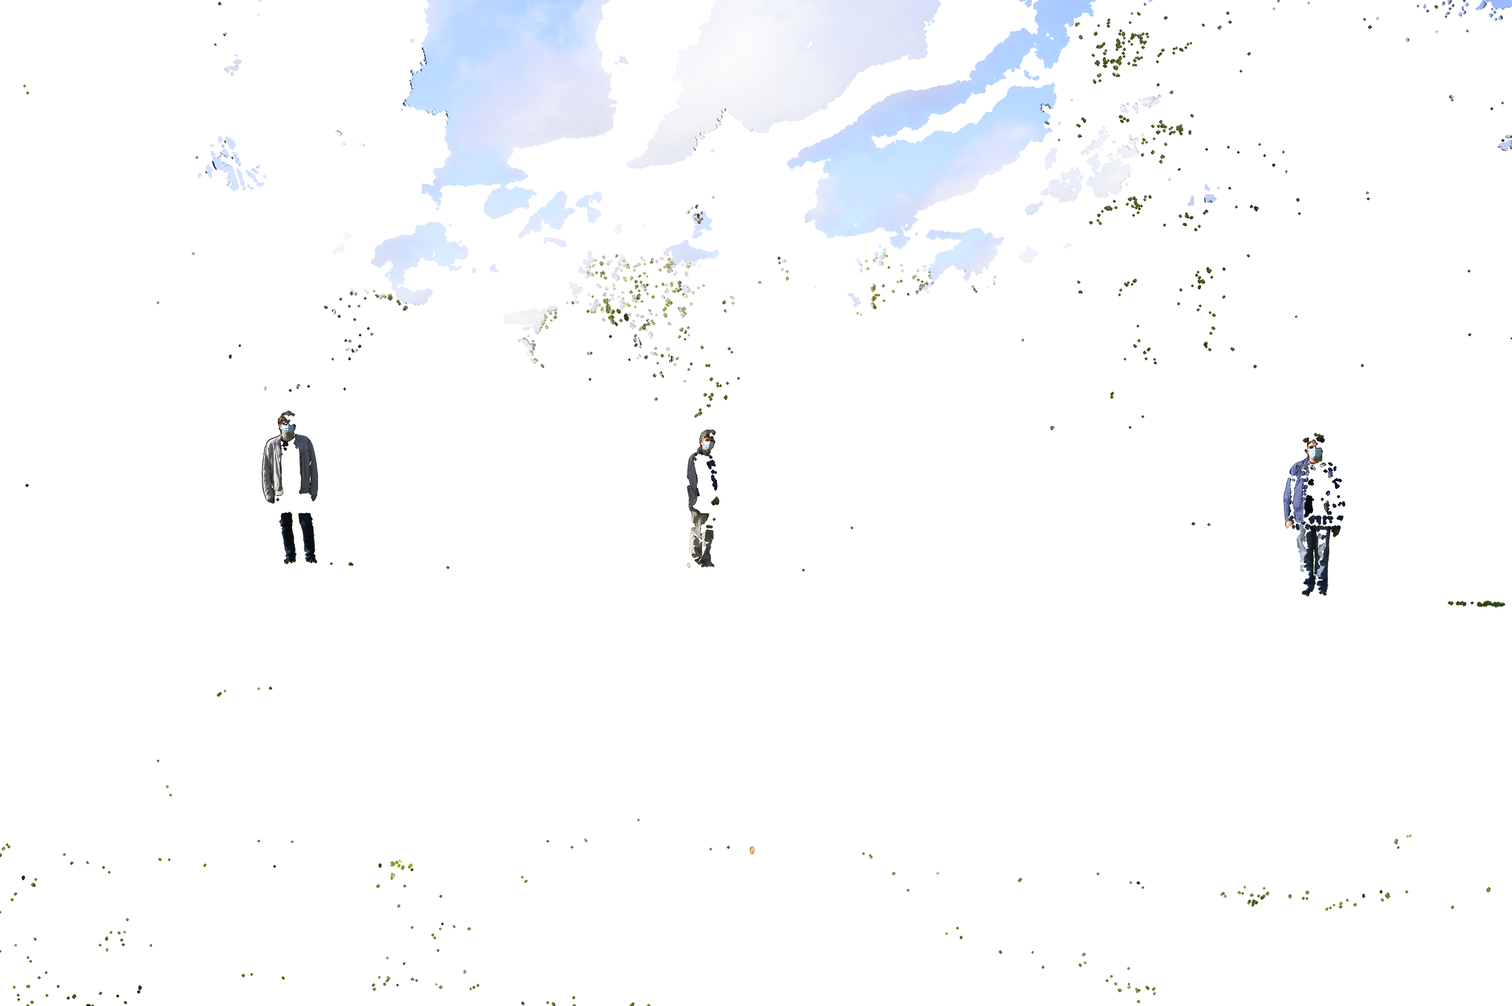
\includegraphics[width=.3\linewidth]{../assets/1512x1006/results_sig1_win5/garden/result_detected_garden_fg_3.png}} &
    \fbox{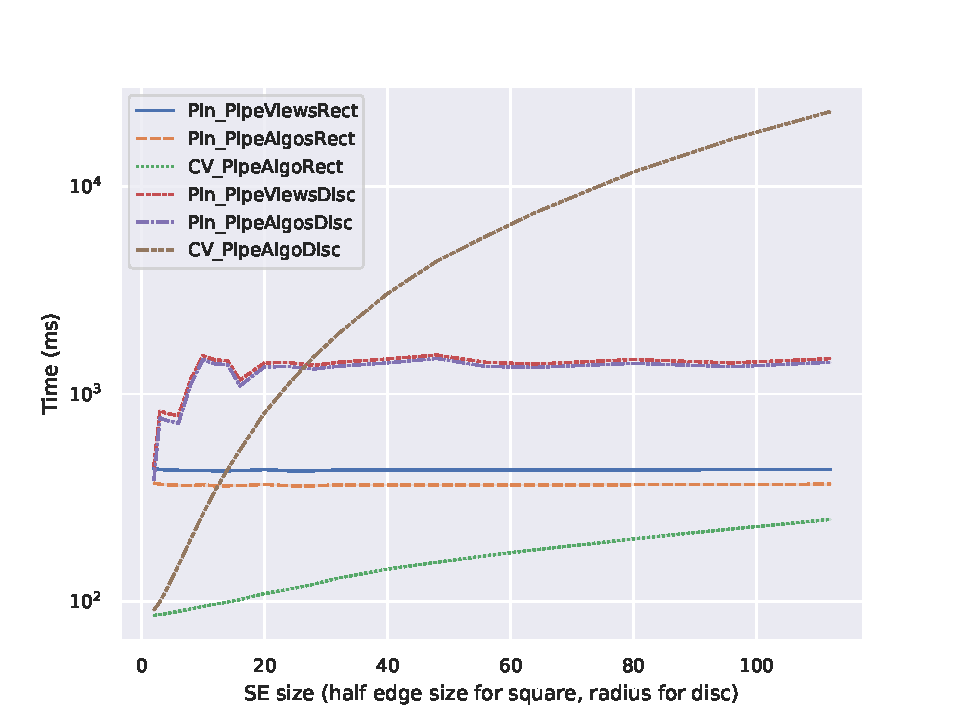
\includegraphics[width=.3\linewidth]{figs/bench/PlnVsOpenCV_bg_sub_3.pdf}}                                          &
    \fbox{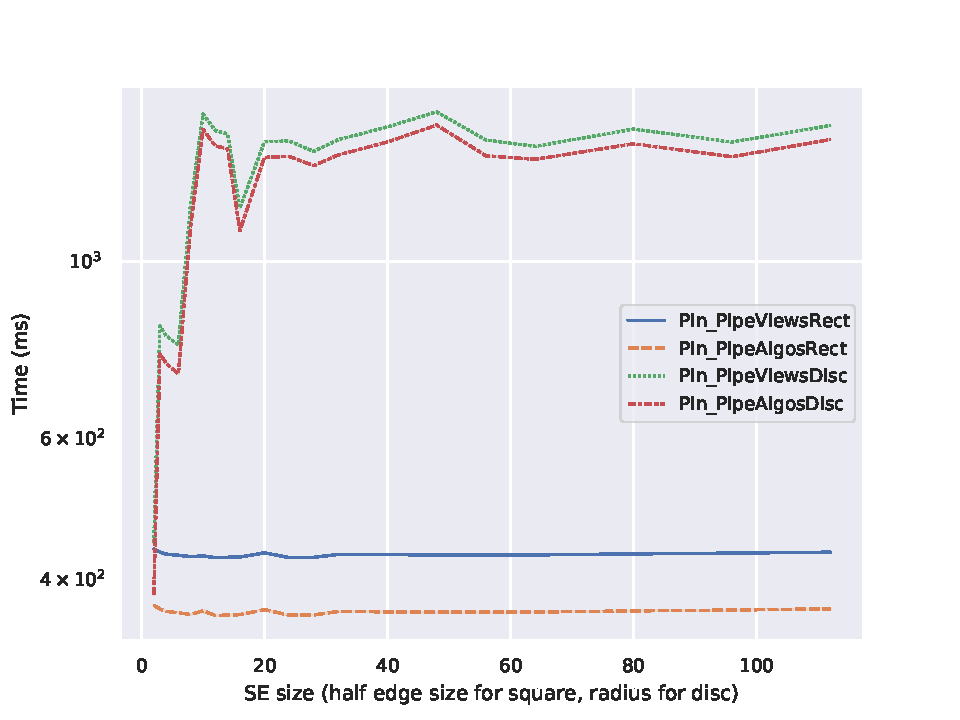
\includegraphics[width=.3\linewidth]{figs/bench/PlnVsOpenCV_bg_sub_pln_3.pdf}}                                                                       \\[5pt]
    \fbox{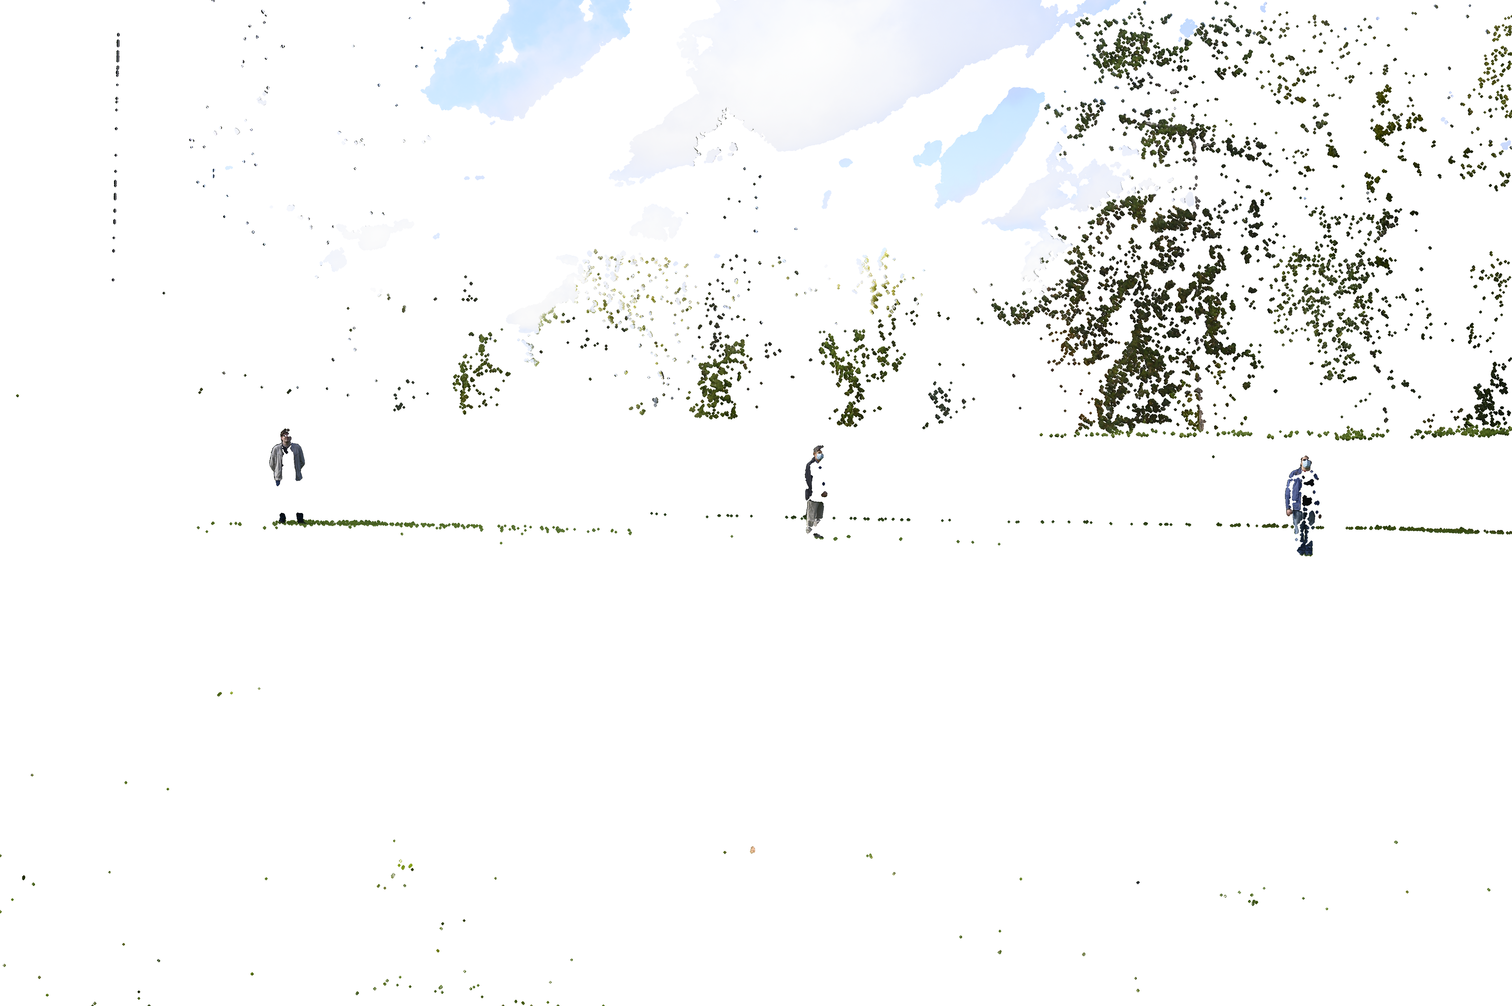
\includegraphics[width=.3\linewidth]{../assets/1512x1006/results_sig1_win5/garden/result_detected_garden_fg_4.png}} &
    \fbox{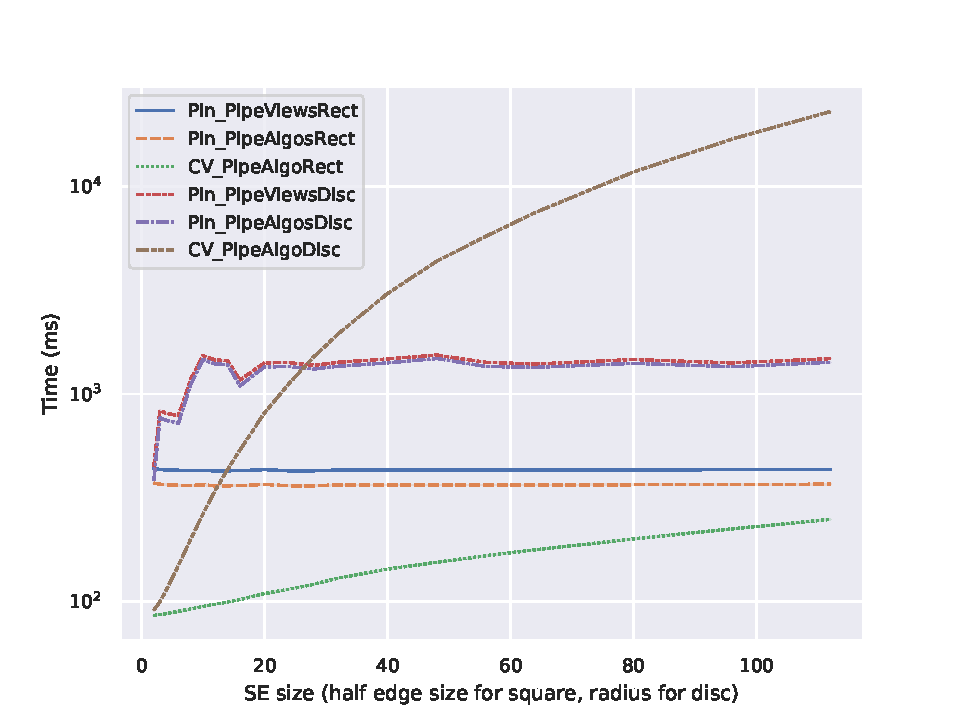
\includegraphics[width=.3\linewidth]{figs/bench/PlnVsOpenCV_bg_sub_4.pdf}}                                          &
    \fbox{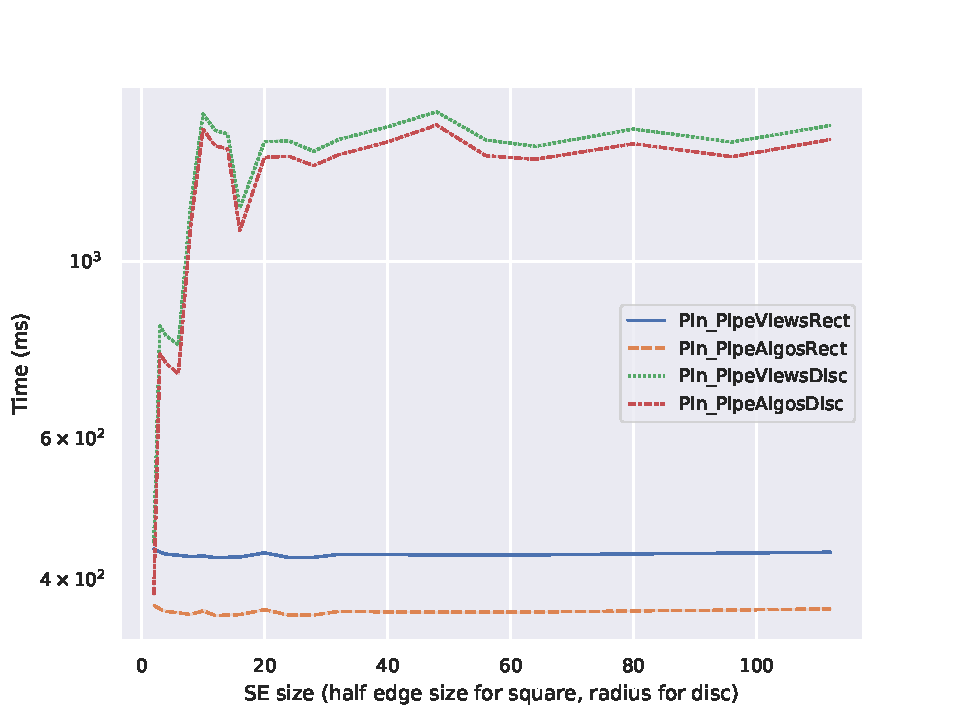
\includegraphics[width=.3\linewidth]{figs/bench/PlnVsOpenCV_bg_sub_pln_4.pdf}}                                                                       \\[5pt]
    \fbox{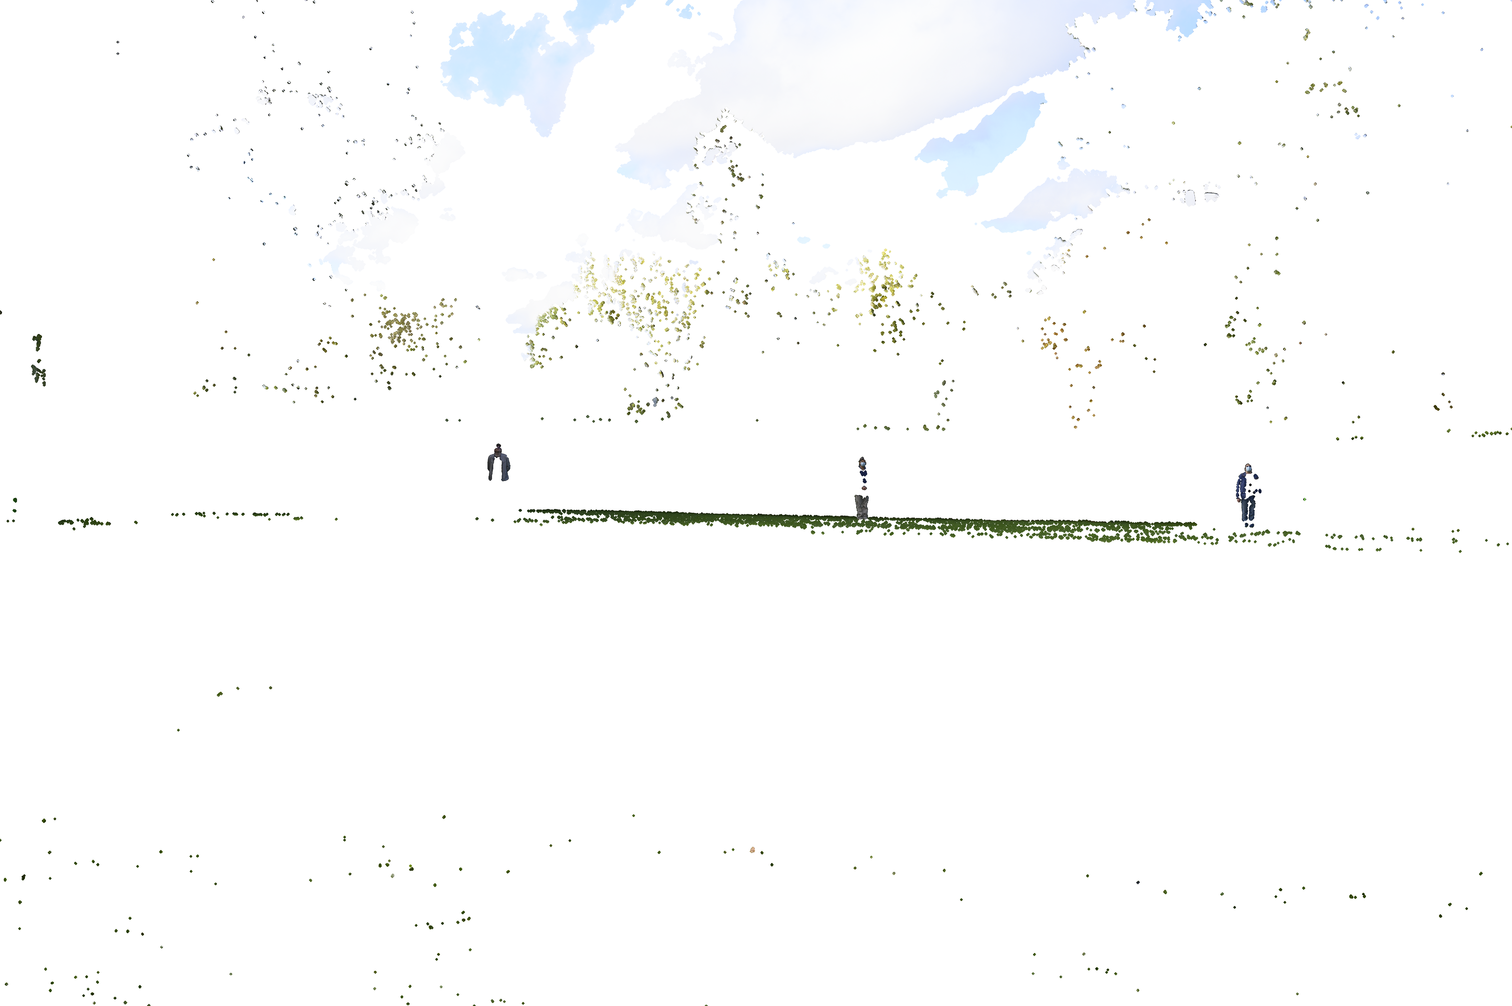
\includegraphics[width=.3\linewidth]{../assets/1512x1006/results_sig1_win5/garden/result_detected_garden_fg_5.png}} &
    \fbox{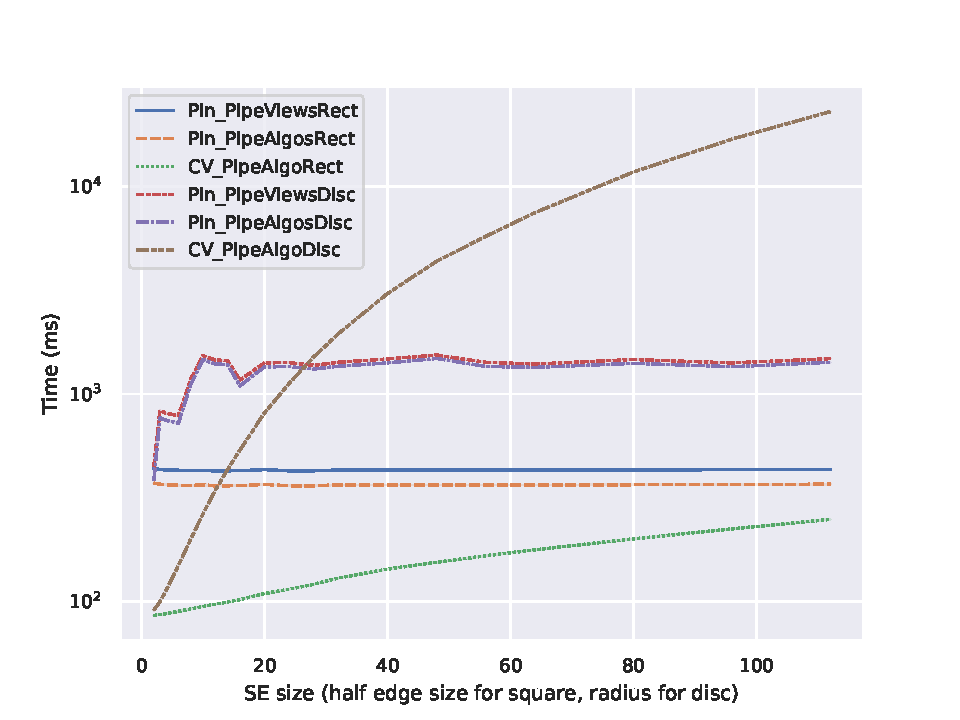
\includegraphics[width=.3\linewidth]{figs/bench/PlnVsOpenCV_bg_sub_5.pdf}}                                          &
    \fbox{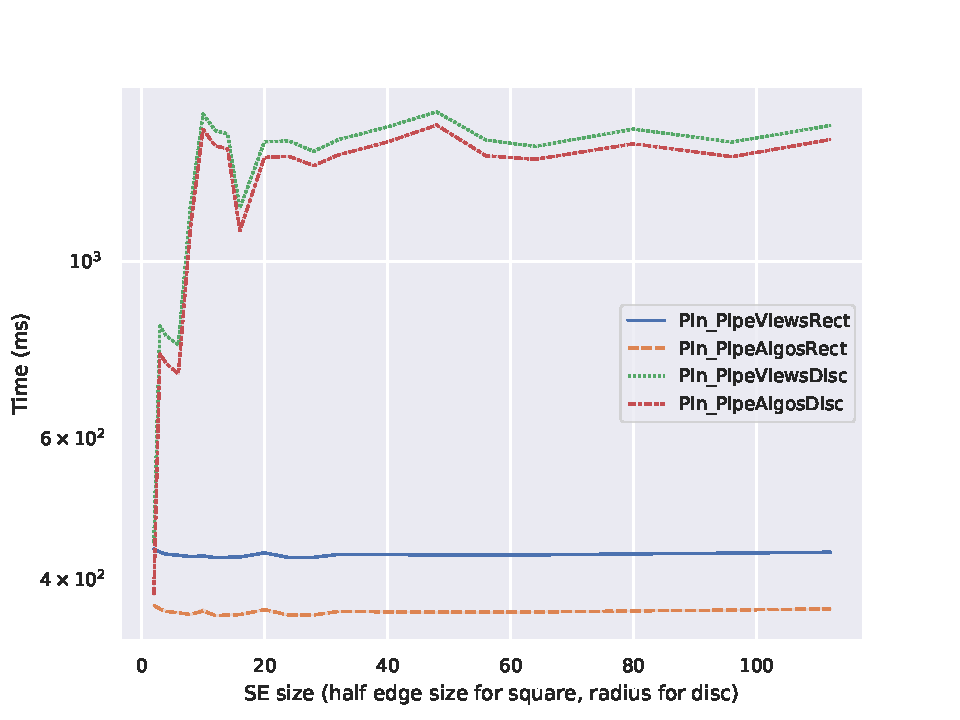
\includegraphics[width=.3\linewidth]{figs/bench/PlnVsOpenCV_bg_sub_pln_5.pdf}}
  \end{tabular}

  \caption{Background detection: garden results.}
  \label{fig:bg_sub.garden.benchmarks}
\end{figure}

\paragraph{Set \#3: pathway} Finally, we have run our algorithm on a last original set of image presented in
figure~\ref{fig:bg_sub.pathway.restults}.

\begin{figure}[tbh]
  \centering
  \begin{tabular}{cccc}
    Background
                                                                                      & Candidate & Result                      \\[5pt]
    \fbox{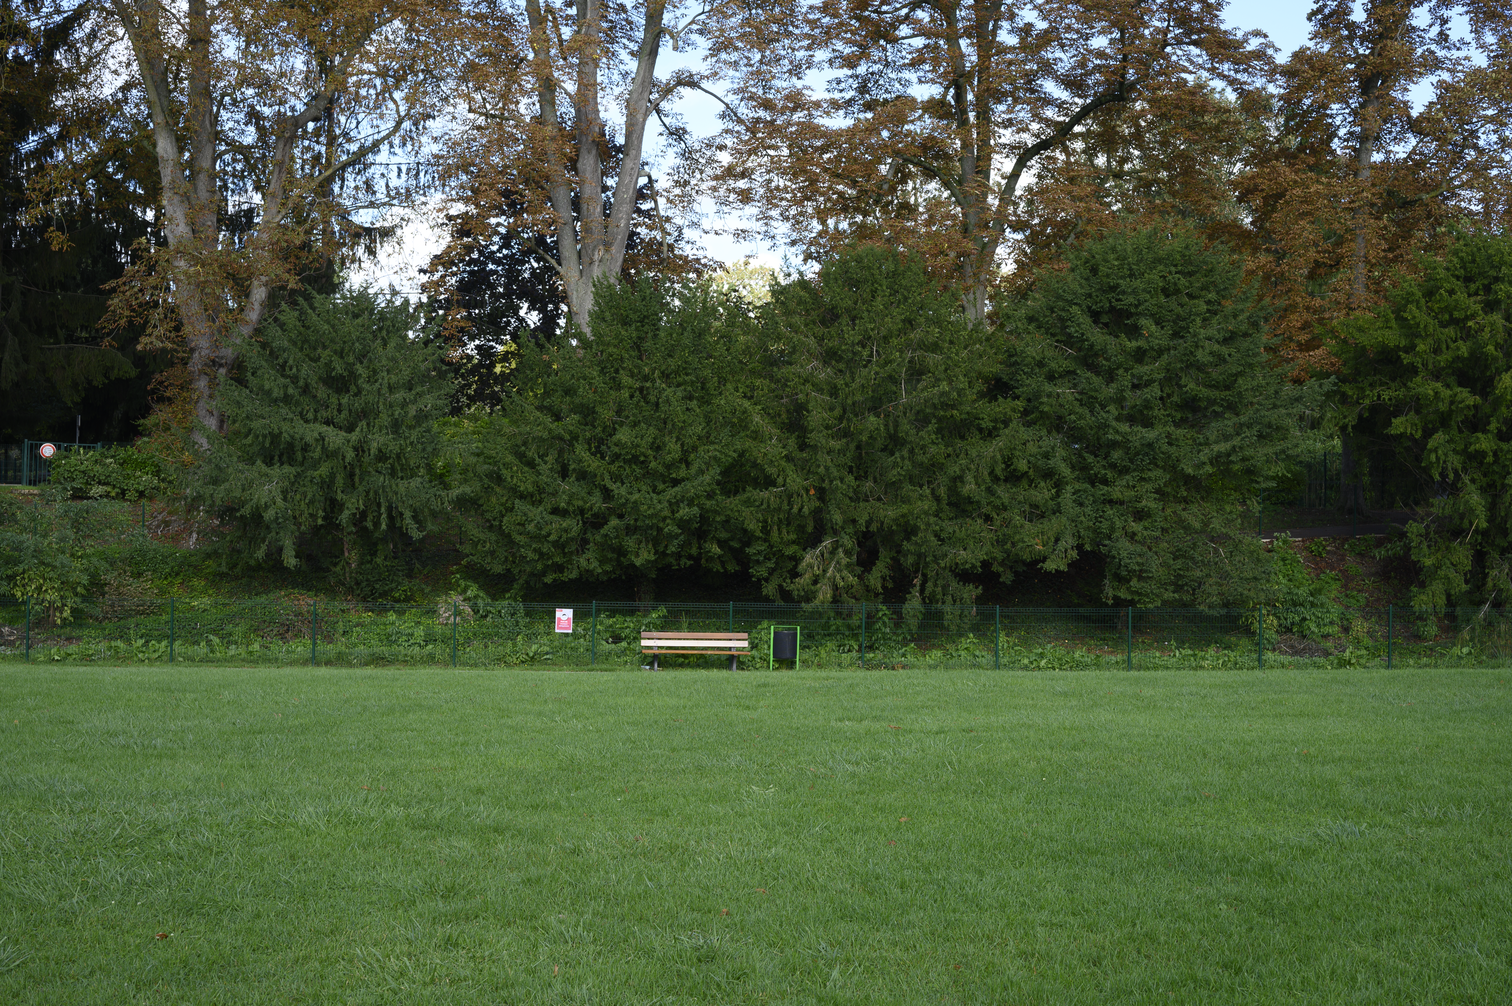
\includegraphics[width=.3\linewidth]{../assets/1512x1006/pathway_bg.png}}   &
    \fbox{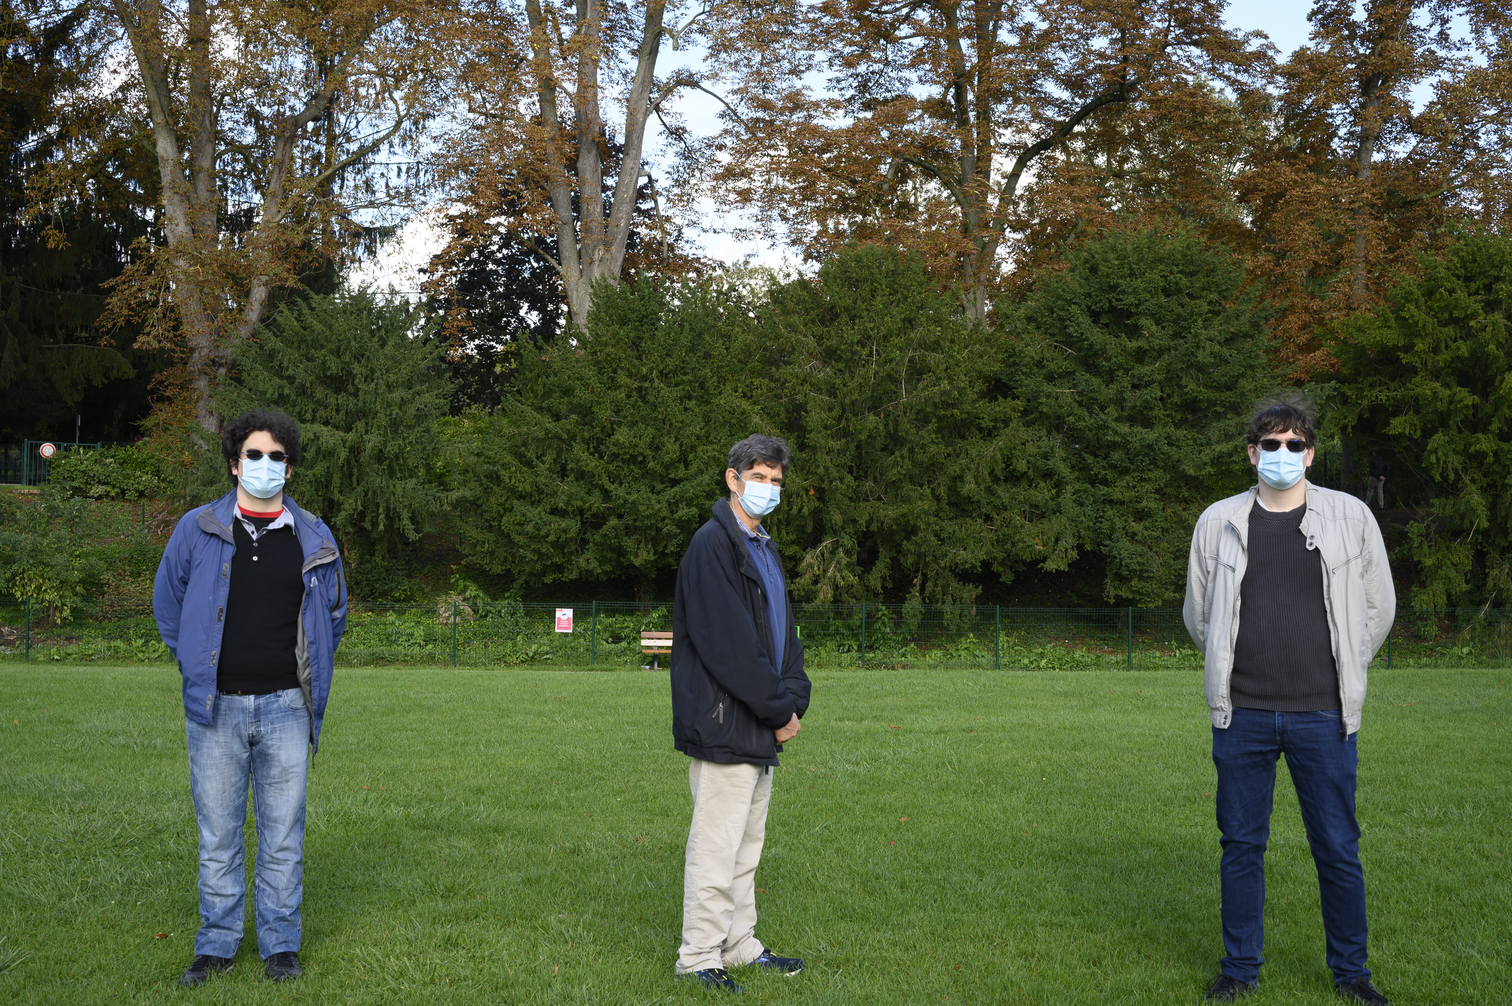
\includegraphics[width=.3\linewidth]{../assets/1512x1006/pathway_fg_1.png}} &
    \fbox{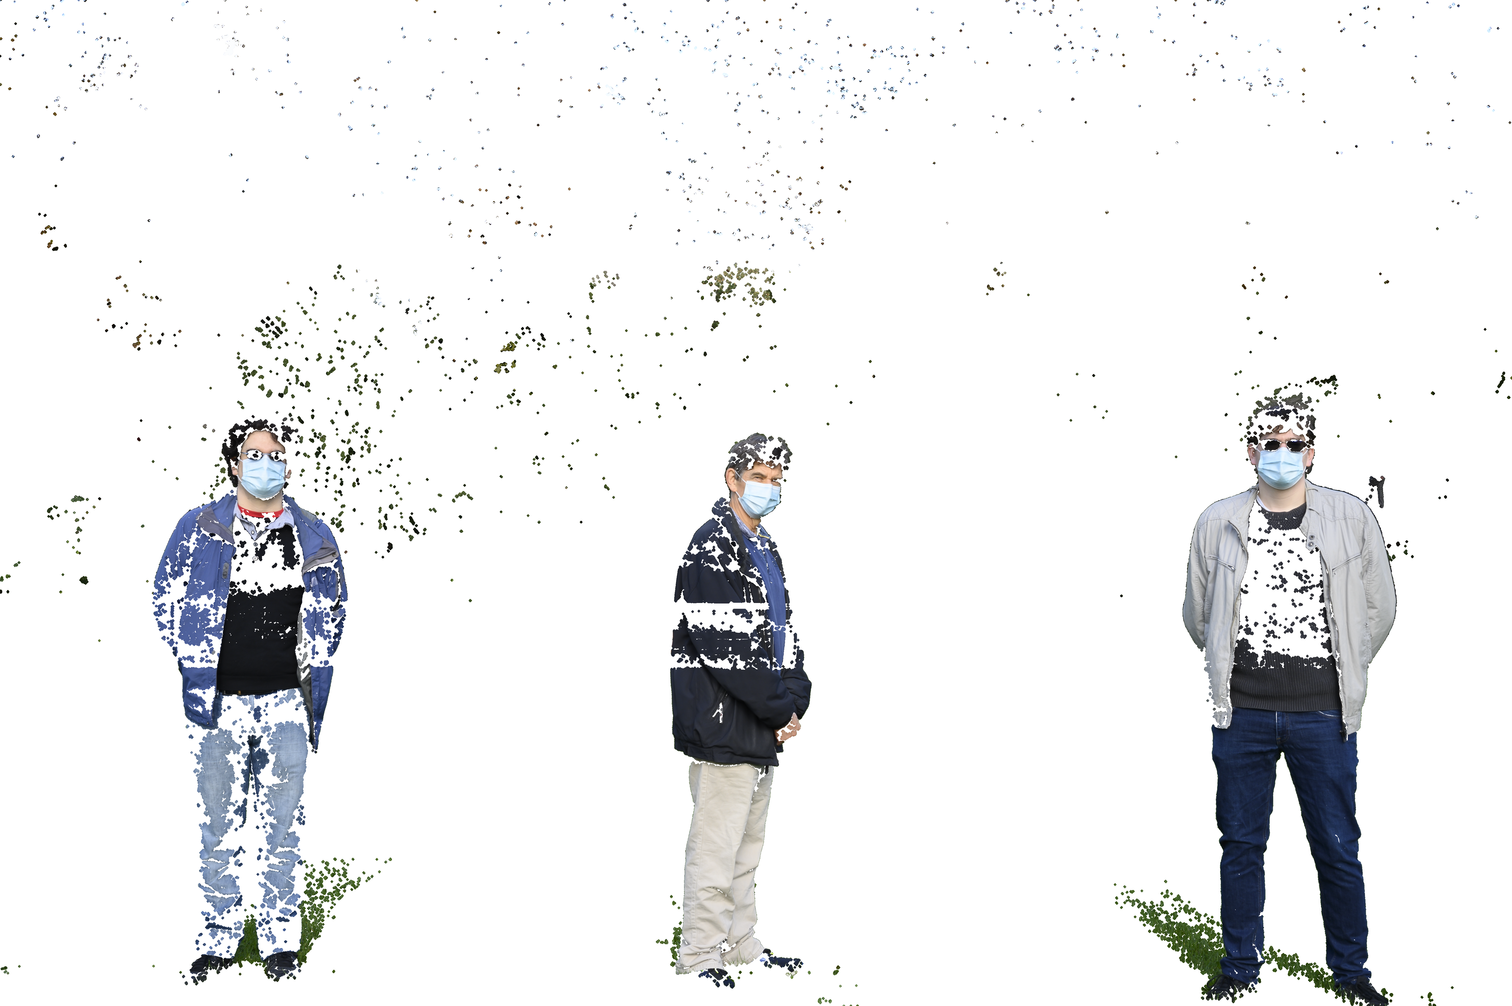
\includegraphics[width=.3\linewidth]{../assets/1512x1006/results_sig1_win5/pathway/result_detected_pathway_fg_1.png}} \\[5pt]
    \fbox{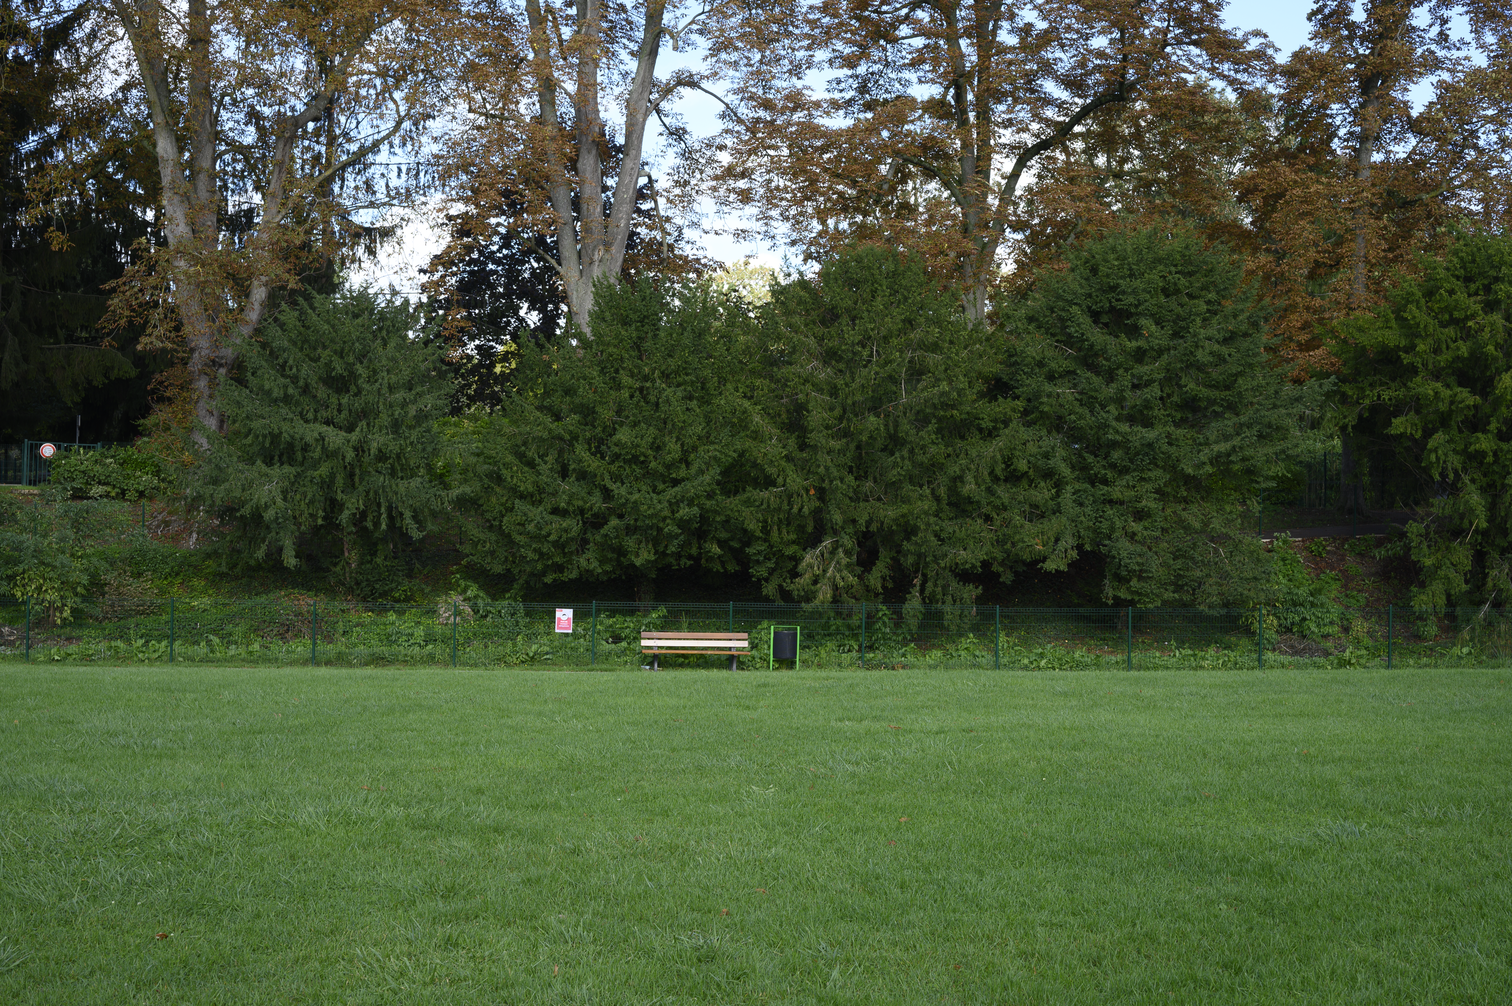
\includegraphics[width=.3\linewidth]{../assets/1512x1006/pathway_bg.png}}   &
    \fbox{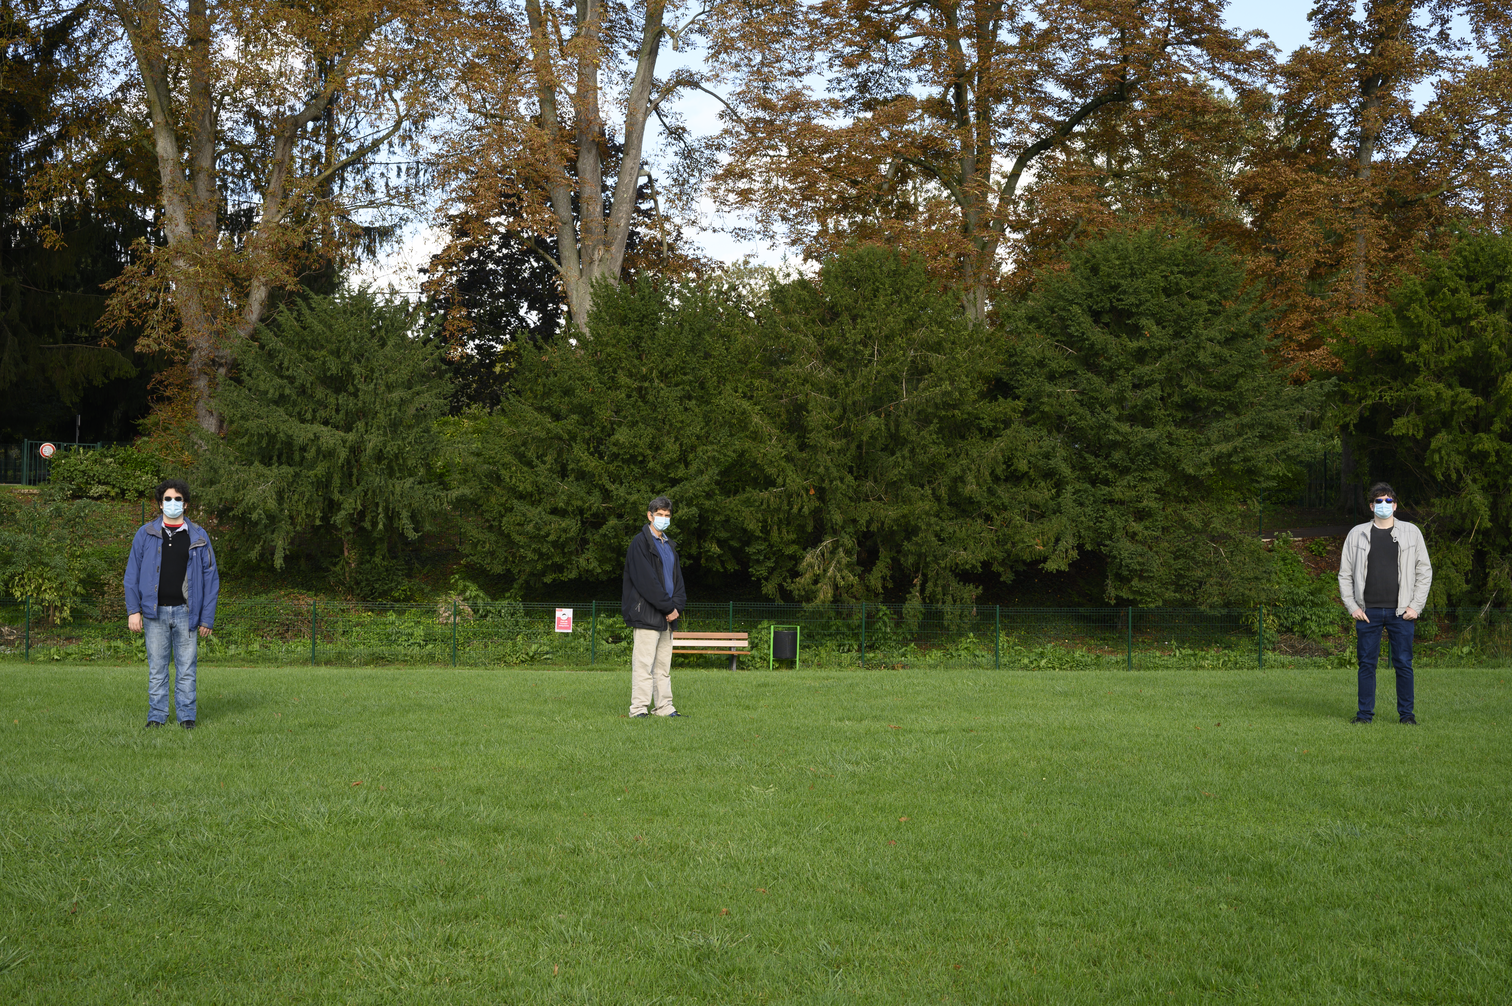
\includegraphics[width=.3\linewidth]{../assets/1512x1006/pathway_fg_2.png}} &
    \fbox{\includegraphics[width=.3\linewidth]{../assets/1512x1006/results_sig1_win5/pathway/result_detected_pathway_fg_2.png}} \\[5pt]
    \fbox{\includegraphics[width=.3\linewidth]{../assets/1512x1006/pathway_bg.png}}   &
    \fbox{\includegraphics[width=.3\linewidth]{../assets/1512x1006/pathway_fg_3.png}} &
    \fbox{\includegraphics[width=.3\linewidth]{../assets/1512x1006/results_sig1_win5/pathway/result_detected_pathway_fg_3.png}} \\[5pt]
    \fbox{\includegraphics[width=.3\linewidth]{../assets/1512x1006/pathway_bg.png}}   &
    \fbox{\includegraphics[width=.3\linewidth]{../assets/1512x1006/pathway_fg_4.png}} &
    \fbox{\includegraphics[width=.3\linewidth]{../assets/1512x1006/results_sig1_win5/pathway/result_detected_pathway_fg_4.png}}
  \end{tabular}

  \caption{Background detection: pathway results.}
  \label{fig:bg_sub.pathway.restults}
\end{figure}

The breakdown of the benchmarks corresponding to this original set is presented in the
figures~\ref{fig:bg_sub.pathway.benchmarks}.

\begin{figure}[tbh]
  \centering
  \begin{tabular}{cccc}
    Result                                                                                                                      & Benchmark & Benchmark Pln only \\[5pt]
    \fbox{\includegraphics[width=.3\linewidth]{../assets/1512x1006/results_sig1_win5/pathway/result_detected_pathway_fg_1.png}} &
    \fbox{\includegraphics[width=.3\linewidth]{figs/bench/PlnVsOpenCV_bg_sub_6.pdf}}                                            &
    \fbox{\includegraphics[width=.3\linewidth]{figs/bench/PlnVsOpenCV_bg_sub_pln_6.pdf}}                                                                         \\[5pt]
    \fbox{\includegraphics[width=.3\linewidth]{../assets/1512x1006/results_sig1_win5/pathway/result_detected_pathway_fg_2.png}} &
    \fbox{\includegraphics[width=.3\linewidth]{figs/bench/PlnVsOpenCV_bg_sub_7.pdf}}                                            &
    \fbox{\includegraphics[width=.3\linewidth]{figs/bench/PlnVsOpenCV_bg_sub_pln_7.pdf}}                                                                         \\[5pt]
    \fbox{\includegraphics[width=.3\linewidth]{../assets/1512x1006/results_sig1_win5/pathway/result_detected_pathway_fg_3.png}} &
    \fbox{\includegraphics[width=.3\linewidth]{figs/bench/PlnVsOpenCV_bg_sub_8.pdf}}                                            &
    \fbox{\includegraphics[width=.3\linewidth]{figs/bench/PlnVsOpenCV_bg_sub_pln_8.pdf}}                                                                         \\[5pt]
    \fbox{\includegraphics[width=.3\linewidth]{../assets/1512x1006/results_sig1_win5/pathway/result_detected_pathway_fg_4.png}} &
    \fbox{\includegraphics[width=.3\linewidth]{figs/bench/PlnVsOpenCV_bg_sub_9.pdf}}                                            &
    \fbox{\includegraphics[width=.3\linewidth]{figs/bench/PlnVsOpenCV_bg_sub_pln_9.pdf}}
  \end{tabular}

  \caption{Background detection: pathway results.}
  \label{fig:bg_sub.pathway.benchmarks}
\end{figure}

For small structuring elements ($radius < 15$), OpenCV is faster thanks to its handwritten code optimization. However,
when the size of the structuring elements increase, so does the execution time, especially for structuring elements
shaped as discs. We can see that the way OpenCV decomposes its structuring elements is not efficient for a disc whereas
it is very efficient for a rectangle. Pylene, on the other hand has a starting cost higher even for small structuring
elements but is extremely stable over the increase of structuring elements' size. Indeed, the only variation is seen
when we are working with the disc shape and this variation stabilise for larger size. For a disc whose $radius > 25$,
Pyelene will be faster than OpenCV.

When looking at the performance of algorithms expressed in term of views, we can see that expressing an algorithm in
term of view incurs a very small overhead that stays constant and stable over the increase of structuring elements'
radius. Furthermore, it does not show on the graphics but the memory consumption is reduced when using views. Indeed,
more computation is done on the fly and the image is copied less during the algorithm. This implies that caching values
is harder when using views which may explain the overhead.

% \chapter*{Material about views}
% 
% 
% \section*{Introducing range-based image traversing}
% \label{sec.range.traversing}
% 
% Previously in Milena~\cite{levillain.2009.ismm} we had a very customized way of traversing images: macro-based. It aimed
% at hiding the complexity of such a task while loosing as little performance as possible. For example, the dilation
% algorithm was written this way:
% 
% \begin{minted}{c++}
%   template<class I, class SE>
%   mln_concrete(I) dilate(const I& f, const SE& se)
%   {
%     mln_concrete(I) g;
%     initialize(g, f);
%     mln_piter(I) p(f.domain());
%     mln_qiter(SE) q(se, p);
%     for_all(p) // for all p in f domain
%     {
%       mln_value(I) v = f(p);
%       for_all(q) // for all q in se(p)
%         if(f.has(q) and f(q) > v)
%           v = f(q);
%       g(p) = v;
%     }
%     return g;
%   }
% \end{minted}
% 
% In this code \texttt{mln\_concrete}, \texttt{mln\_piter}, \texttt{mln\_qiter}, \texttt{for\_all} and \texttt{mln\_value}
% are all macros aiming at hiding the underlying complexity. Our goal is to replace those macros with existing C++ core
% language code to improve the user experience as well as ease the maintenance, contribution and further improvement of
% the library. Nowadays, a tool named range (and especially Eric Niebler's range-v3) allow seamless traversing of an
% image. For instance, we can rewrite the above algorithm this way:
% 
% \begin{minted}{c++}
%   template<class I, class SE>
%   image_concrete_t<I> dilate(const I& f, const SE& se)
%   {
%     auto g = f.concretize();
%     auto supr = accu::supremum<image_value_t<I>>();
%     for(auto [f_px, g_px] : zip(f.pixels(), g.pixels()))
%     {
%       for(auto qx : se(f_px))
%         supr.take(qx.val());
%       g_px.val() = supr.result();
%     }
%     return g;
%   }
% \end{minted}
% 
% Here we have a much more efficient code that, in theory, enables compiler optimizations such as vectorization or inner
% loops unrolling. But through benchmarking, we have learned that this solution doesn't mix well with the multidimensional
% nature of images. The issue originates from the fact that we have no way to explicitly say in the code that the
% multidimensional range is made of chunk of contiguous rows of memory. Indeed, for each element we have to compute an
% index originating from potentially $N$ dimensions. This disables critical optimizations such as vectorization.
% 
% We solved this problem by augmenting range-v3's ranges with our own multidimensional ranges. Indeed, we only need to
% have contiguity on the last dimension to provide the compiler code it can optimize. Which means that each for-loop that
% traverses the whole n-dimensional image can be transformed into a double for-loop whose inner loop is guaranteed to be a
% contiguous row. This way we have now an outer range as well as an inner range, as illustrated in
% figure~\ref{fig.inner.outer.range}.
% 
% \begin{figure}[htbp]
%   \centering
%   \subcaptionbox{}{\includegraphics[width=.48\linewidth]{figs/linear_rng}}
%   \subcaptionbox{}{\includegraphics[width=.48\linewidth]{figs/segmented_rng}}
%   \caption{Range-v3's ranges (a) vs. multidimensional ranges (b).}
%   \label{fig.inner.outer.range}
% \end{figure}
% 
% Thanks to this new design we can now rewrite our algorithm with a double for-loop for the image traversing. Hopefully it
% stays really similar to what one would be used to when working with the classical two dimension image. As an example, we
% can rewrite the dilation algorithm this way:
% 
% \begin{minted}{c++}
%   template<class I, class SE>
%   image_concrete_t<I> dilate(const I& f, const SE& se)
%   {
%     auto g = f.concretize();
%     auto supr = accu::supremum<image_value_t<I>>();
%     auto zipped_pixels = zip(f.pixels(), g.pixels());
%     for(auto&& row : ranges::rows(zipped_pixels))
%       for(auto [f_px, g_px] : row)
%       {
%         for(auto qx : se(f_px))
%           supr.take(qx.val());
%         g_px.val() = supr.result();
%       }
%     return g;
%   }
% \end{minted}
% 
% The highlight of this code is the usage a new tool: \texttt{ranges::rows} to bring out an inner range (contiguous) from
% the multidimensional outer range.
% 
% \clearpage
% 
% \begin{itemize}
%   \item origine, parallèle avec range-v3
%   \item Value/Ref semantics des images
%   \item Comment préserver les propriétés
%   \item Évaluation paresseuse
%   \item Composabilité/chaînage
%   \item ...
%   \item Performances + Bench
% \end{itemize}